\documentclass[main.tex]{subfiles}
\begin{document} 
\section{Recent Advances and Exact Results}
In recent decades there has been huge interest towards the study and classification of quantum field theories in various dimensions. One motivation for this study is the desire to understand the `landscape' of all permissible quantum field theories. Some regions of this `landscape' are somewhat understood, for example Yang-Mills theories at high energies (UV). This is largely due to the framework for organising the perturbation theory introduced by Feynman in the 1940's. The importance of perturbation theory cannot be overstressed; high precision tests of the electron g-factor from the LHC agree with the theoretical predicitions of the standard model up to 14 digits of precision \cite{hanneke2008new}.
Conversely, relatively little is known about about the low energy (IR) behaviour of such theories because said perturbative techniques breaks down.  This is because because in Yang-Mills theories the coupling is a function of the energy scale and the coupling is said to `run' with the energy scale.  Yang-Mills theories are weakly coupled in the UV but as we flow to the IR the coupling grows and non-perturbative phenomena, such as colour confinement and instantons, become relevant; they are therefore said to be \textit{asymptotically free}.  Indeed, the perturbative expansion is an asymptotic expansion in the coupling and convergence of the series requires the inclusion of non-perturbative effects.  Moreover, it has become clear that the landscape of quantum field theories also contains a vast number of theories that cannot be understood via the standard local Lagrangian/path integral formulation found in introductory QFT textbooks.  

If we restrict our attention to theories with a certain amount of \textit{supersymmetry} much more can be understood.  This may be seen as a lowering of ambition (all though still an incredibly lofty undertaking) because supersymmetry is either yet to be discovered or may not exist in nature. Nevertheless, supersymmetric theories offer examples of consistent quantum field theories.  Supersymmetric theories are far from non-trivial and also offer many of the interesting phenomena expected in non-supersymmetric theories, such as confinement, but in a more constrained and controllable framework.

Supersymmetry is a fermionic spacetime symmetry which pairs bosons and fermions together.  The presence of this additional symmetry constrains the dynamics of the theory and can often mean that supersymmetric theories are far more tractable to study.  In comparison to non-supersymmetric theories, where relatively little is known outside of the perturbative regime, for supersymmetric theories there are by now a large number of results and many of them will be reviewed and discussed within this thesis.  

As previously discussed, for non-supersymmetric theories, we, so far, have a rather limited toolkit with which to study such theories; the main tool being perturbation theory.\footnote{For very special (highly symmetrical) non-supersymmetric QFTs, such as topological, conformal or integrable QFTs we have other tools and can often compute some non-perturbative results or even `solve' the theory.} But, when we restrict our attention to QFTs with some amount of supersymmetry, we can employ a plethora of new tools with which we can access and study non-perturbative effects.  An overview of these tools can be found in \cite{Tachikawa:2013kta,Teschner:2016yzf,Pestun:2016zxk,Tachikawa:2018sae}.  They can often allow us to compute \textit{exact results} for these theories. In other words, observables for the theory which are valid even for the non-perturbative regime.  Much of the computation and study of exact results has so far been dedicated to theories with eight or more supercharges, in four dimensions this is $\mathcal{N}\geq2$ supersymmetry.  Additionally, aided by string/M/F-theoretic techniques, physicists have been able to construct a vast number of so-called \textit{non-Lagrangian} theories.  As we previously mentioned they do not admit a path integral description and usually live as isolated conformal theories.  They can nevertheless sometimes be partially understood using string/M/F-theoretic reasoning and often are related to Lagrangian theories via strong/weak dualities.

\section{Seiberg-Witten Theory}\label{eqn:introSW}
In 1994 Seiberg \& Witten provided one of the first computations of an exact result in a four dimensional gauge theory. They were able to compute the low-energy effective action on the Coulomb branch for four-dimensional $\mathcal{N}=2$ gauge theories based upon a Lie-algebra $\mathfrak{g}$ \cite{Seiberg:1994rs,Seiberg:1994aj} with Cartan subalgebra $\mathfrak{h}$.\footnote{Their original computations were based off of $\mathfrak{g}=\mathfrak{su}(2)$ with $N_f=0,1,\dots,4$ fundamental hypermultiplets or a single adjoint hypermultiplet ($\mathcal{N}=2^*$).  Over the years this has since been generalised to a large number of $\mathcal{N}=2$ theories, see Section 4.5 of \cite{Bhardwaj:2013qia} for an exhaustive list.} These theories are comprised of $\mathcal{N}=2$ vector multiplets and a collection of hypermultiplets.  The on-shell field content of a $\mathcal{N}=2$ vector multiplet is the same as for a $\mathcal{N}=1$ chiral multiplet $\Phi$ (containing a complex scalar $\phi$ and complex Weyl fermion $\psi$), anti-chiral multiplet $\overline{\Phi}$ and $\mathcal{N}=1$ vector multiplet $V$ (Weyl fermion $\lambda$, anti-Weyl fermion $\overline{\lambda}$ and one-form gauge potential $A$) all in the adjoint representation of the gauge algebra.  The field content of the hypermultiplet in a representation $\mathcal{R}\oplus\overline{\mathcal{R}}$, for $\mathcal{R}$ pseudo-real, is two half-hypermultiplets $(Q,\widetilde{Q})$ in the representations $\mathcal{R}$ and $\overline{\mathcal{R}}$.  A half-hypermultiplet is a $\mathcal{N}=1$ chiral multiplet.  The decomposition $\mathfrak{g}=\oplus_i\mathfrak{g}_i$, with $\mathfrak{g}_i$ either simple or $\mathfrak{u}(1)$, induces the decomposition $\mathcal{R}=\oplus \mathcal{R}_{i,a}$ with $\mathcal{R}_{i,a}$ irreducible.  The one-loop beta function associated to the factor $\mathfrak{g}_i$ is then
\begin{equation}
\beta_i=E\frac{d}{dE}g_i=-\frac{g^3}{(4\pi)^2}b_i\,,\quad b_i=2h^{\vee}(\mathfrak{g}_i)-\sum_{a}c_2(\mathcal{R}_{i,a})\prod_{j\neq i}\dim_{\mathbb{R}}\mathcal{R}_{j,a}\,.
\end{equation}
Here $h^{\vee}({\mathfrak{g}})$ denotes the dual Coxeter number of $\mathfrak{g}$ and $c_2(\mathcal{R})$ the quadratic Casimir (Dynkin index) of the representation $\mathcal{R}$.

Due to powerful non-renomalisation theorems \cite{Grisaru:1979wc,Seiberg:1994bp,Seiberg:1993vc,Seiberg:1988ur} this is an exact statement valid to all orders in perturbation theory.  In order for the theory to be UV-complete we must have that $b_i\geq0$.  If each $b_i=0$ then the theory is (perturbatively) conformal.

Such a theory has a moduli space of supersymmetric vacua $\mathbf{M}$.  This is the space of zero-energy configurations of the theory and is schematically defined as
\begin{equation}\label{eqn:Modspacedef}
\mathbf{M}:=\left\{\phi,q,\widetilde{q}\middle|V(\phi,q,\widetilde{q})=0\right\}/G\,,
\end{equation}
here $\phi,q,\widetilde{q}$ denote the scalar components of $\Phi,Q,\widetilde{Q}$, respectively and $V(\phi,q,\widetilde{q})$ denotes the scalar potential.
The Coulomb branch $\mathbf{CB}\subset \mathbf{M}$ for a four dimensional $\mathcal{N}=2$ theory is a particular submanifold reached by allowing constant vevs for $\langle\phi\rangle=a\in\mathfrak{h}$ while setting to zero vevs for $\langle Q\rangle=\langle\widetilde{Q}\rangle=0$.  The Coulomb-branch is therefore parametrised by the generators $u_{i=1,2,\dots\rank\mathfrak{g}}$ of the ring of $\mathfrak{g}$-invariant polynomials in the $\phi$ and so $\dim_{\mathbb{C}} \mathbf{CB}=\rank\mathfrak{g}$.  By gauge transformation we can take $a$ to be diagonal and therefore the gauge algebra $\mathfrak{g}$ is broken down to the stabiliser subalgebra of $\mathfrak{g}$ with respect to $a$.  This is simply the Cartan subalgebra $\mathfrak{h}\subset\mathfrak{g}$, i.e.  the Lie algebra of $C_{G}(a)$.  Therefore, in the IR, we will have an abelian gauge theory based on gauge group $\exp\mathfrak{h}\iso U(1)^{\rank\mathfrak{g}}$.  Due to $\mathcal{N}=2$ supersymmetry the form of the effective action of this theory is highly constrained and depends only on a single holomorphic function $\mathcal{F}(a)$ called the \textit{prepotential} \cite{1988PhLB..206...75S}.  The effective action in $\mathcal{N}=1$ language reads
\begin{gather}
S_{\text{eff}}=\frac{1}{4\pi}\Im\left[\int \extd^4\theta a^D_i\overline{a}_i+\frac{1}{2}\int \extd^2\theta\tau_{ij}\,W_{\alpha}^iW^{\alpha j}\right]\,,\\
 \tau_{ij}(a)=\frac{\partial^2\mathcal{F}(a)}{\partial a^i\partial a^j}\,,\quad a^D_i(a)=\frac{\partial \mathcal{F}(a)}{\partial a^i}\,,\\i,j\in\{1,2,\dots,\rank\mathfrak{g}\}\,.
\end{gather}
The task is then to compute $\mathcal{F}(a)$.  The solution of Seiberg-Witten is that the prepotential is encoded in a pair $(\mathcal{X}_{\{u_i\}},\lambda_{\text{SW}})$, where $\mathcal{X}_{\{u_i\}}$ denotes a Riemann surface of genus $g\geq\rank\mathfrak{g}$ called the Seiberg-Witten curve and $\lambda_{\text{SW}}$ a meromorphic one-form on $\mathcal{X}_{\{u_i\}}$.  There are a family of Riemann surfaces $\mathfrak{X}=\{\mathcal{X}_{\{u_i\}}\}$ realised as a fibration over the moduli space of Coulomb branch vacua $\mathbf{CB}$, which is parametrised by the $u_i$.  At a generic point on $\mathbf{CB}$ specified by the $u_i$ the fiber is $\mathcal{X}_{\{u_i\}}$ and is given in terms of a polynomial $y^2=F(x;u_i,q)$ in two auxiliary variables $x,y$.  We will now sketch the derivation of this result for the case $\mathfrak{g}=\mathfrak{su}(2)$ theory without flavour, as first derived in \cite{Seiberg:1994rs}.  
The first point is to notice that $S_{\text{eff}}$ possesses an $SL(2,\mathbb{Z})$ S-duality group 
\begin{equation}
SL(2,\mathbb{Z})\iso\langle S,T|S^4=1,(ST)^3=1\rangle\iso C_4\ast C_3\,,
\end{equation}
where $C_n$ is the cyclic group $|C_n|=n$ and $\ast$ is the free product.  An explicit realisation is
\begin{equation}
S=\begin{pmatrix}
0&1\\-1&0
\end{pmatrix}\,,\quad T=\begin{pmatrix}
1&1\\0&1
\end{pmatrix}\,.
\end{equation}
An element of $SL(2,\mathbb{Z})$ acts on the vector $(a_D\,\, a)^{\trans}$ in the fundamental representation while it acts on the effective gauge coupling via fractional linear transformation.  In particular $S$ sends $\tau(a)\to\tau_D(a_D)=-1/\tau(a)$.  In the weak coupling one can easily see the appearance of non-trivial monodromies.  The prepotential is \cite{1988PhLB..206...75S} 
\begin{equation}
\mathcal{F}(a)=\frac{\iu}{2\pi}a^2\log\frac{a^2}{\Lambda^2}+\sum_{i=1}^{\infty}c_k\frac{\Lambda^{4i}}{a^{4i}}a^2\,,
\end{equation}
where $\Lambda^4$ is the holomorphic dynamically generated scale.  In the weak coupling $a\gg\Lambda$ and so, (after normalising $u=\tr\phi^2/\Lambda^2$) looping around infinity on the $u$-plane $u\mapsto e^{2\pi\iu}u$ means
\begin{equation}
\begin{aligned}
\begin{pmatrix}
a^D\\a
\end{pmatrix}=\begin{pmatrix}
\partial\mathcal{F}/{\partial a}\\a
\end{pmatrix}\to M_{\infty}\begin{pmatrix}
a^D\\a
\end{pmatrix}=&\begin{pmatrix}
-1&2\\0&-1
\end{pmatrix}\begin{pmatrix}
a^D\\a
\end{pmatrix}\\
=&S^2T^{-2}\begin{pmatrix}
a^D\\a
\end{pmatrix}\,.
\end{aligned}
\end{equation}
Due to the R-symmetry $u\mapsto-u$ Seiberg and Witten conjectured that the $u$-plane has three singular points, at $u=\infty,+1,-1$.  The monodromy at $u=+1$ can be determined by appealing to the $SL(2,\mathbb{Z})$ duality.  By applying an $S$-transformation $a^D$ becomes the good coordinate in which to write down the effective action in terms of.  Therefore, around the point $u=+1$, $a^D$ is a good coordinate and $a^D\sim b(u-1)$ for a constant $b$.  Around this point the one-loop beta function shows $\tau^D\simeq-\frac{\iu}{\pi}\log a^D$ and so
\begin{equation}
\begin{aligned}
a(u)&=-\int\tau^D\,da^D\simeq a(u=1)+\frac{\iu}{\pi}a^D\log a^D\\
&\simeq a(u=1)+\frac{\iu}{\pi}b(u-1)\log(u-1)\,.
\end{aligned}
\end{equation}
The monodromy around $u=1$ is therefore
\begin{equation}
\begin{pmatrix}
a^D\\a
\end{pmatrix}\to M_1\begin{pmatrix}
a^D\\a
\end{pmatrix}=\begin{pmatrix}
1&0\\-2&1
\end{pmatrix}\begin{pmatrix}
a^D\\a
\end{pmatrix}=ST^{2}S^{-1}\begin{pmatrix}
a^D\\a
\end{pmatrix}\,.
\end{equation}
The monodromy at $u=-1$ can now easily be computed by demanding
\begin{equation}
M_{-1}=M_1^{-1}M_{\infty}\,.
\end{equation}
If one supplements $M_1,M_{\infty}$ with $-\mathbb{I}$ ($u$ is invariant under $a\to-a$) then it is not too hard to show that those matrices generate the group $\Gamma(2)\subset SL(2,\mathbb{Z})$ where
\begin{equation}
\Gamma(n)=\left\{\begin{pmatrix}
a&b\\c&d
\end{pmatrix}\in SL(2,\mathbb{Z})\middle|a,d=1\bmod n\,,b,c=0\bmod n\right\}\,,
\end{equation}
is the principal congruence subgroup of level $n$ in $SL(2,\mathbb{Z})$.
The solution of the model is therefore to specify the the modular curve $\mathfrak{X}=X(2)=\mathbb{H}/\Gamma(2)$ which can be explicitly written down as as the set of a 1-parameter family of curves $\mathfrak{X}=\{\mathcal{X}_u\}$
\begin{equation}
\mathcal{X}_u:\quad y^2=F(x;u)=(x-u)(x-1)(x+1)\,.
\end{equation}
Recall that we have normalised $u=\tr\phi^2/\Lambda^2$. Choosing a basis $\{A,B\}$ for the $2\rank\mathfrak{g}=2$ independent one-cycles the effective action is computed via the integrals
\begin{equation}
a^i=\int_{A_i}\lambda_{\text{SW}}\,,\quad a^D_i=\int_{B_i}\lambda_{\text{SW}}\,.
\end{equation}
See also Appendix \ref{Chap:AppEllcurve} for more information.  As pointed out in \cite{Seiberg:1994aj,Intriligator:1994sm} the Seiberg-Witten technology may also, in part, be applied to certain theories with only $\mathcal{N}=1$ supersymmetry.  In particular, if the $\mathcal{N}=1$ theory has a Coulomb phase in which the effective action is that of an abelian gauge theory the Seiberg-Witten technology may be applied in order to compute the effective superpotential $W$.  On the other hand the K\"aher potential (which is fixed in terms of $\mathcal{F}(a)$ for $\mathcal{N}=2$ theories, $K=\Im \partial_{a^i} \mathcal{F}\overline{a}_i$) is left unfixed. We investigate this in Chapter \ref{Chap:SkCurves}.

\section{Instantons}\label{Chap:AppInstADHM}
In the last decades much progress has been made towards understanding the non-perturbative (exact) aspects of Yang-Mills theories.  One particular class of solutions to the Yang-Mills equations are called \textit{instantons}.  Yang-Mills instantons are, by definition, solutions of the classical field equations on a Riemannian manifold with finite action.  Reviews of Yang-Mills instantons can be found in \cite{Belitsky:2000ws,Tachikawa:2014dja,Dorey:2002ik,Tong:2005un} while a more mathematical treatment may be found in \cite{Nakajima:2003uh}.

We will consider pure Yang-Mills theory in $d=4$ dimensions based on a Lie algebra $\mathfrak{g}$ on an orientable Riemannian manifold $\mathcal{M}$ with metric $g$ and volume form $\omega\in\Omega^d(\mathcal{M})$.  This is a theory of vector bundles $V\to \mathcal{M}$ equipped with connection $\nabla$ with curvature $F=\ad_{\nabla}\nabla\in\mathfrak{g}\otimes \Omega^2(\mathcal{M})$ associated to principal $G$-bundles $P\to \mathcal{M}$ where $G$ is a connected Lie group of rank $r$ with Lie algebra $\mathfrak{g}$.  This theory has action
\begin{equation}
S=-\frac{1}{2g^2}\int_{\mathcal{M}}\tr F\wedge \star F=-\frac{1}{2g^2}\int_{\mathcal{M}}\tr \langle F,F\rangle\, \omega\,,
\end{equation}
here $\star$ denotes the Hodge star on $\mathcal{M}$. The \textit{Yang-Mills equations} are then
\begin{equation}\label{eqn:YMequations}
\nabla \star F=0\,.
\end{equation}
Recalling that $\star^2=(-1)^{p(d-p)}$ on $p$-forms we can write
\begin{equation}
\tr\langle F,F\rangle=\frac{1}{2}\tr\langle F\pm\star F,F\pm\star F\rangle\mp\tr\langle F,\star F\rangle\geq \mp\tr\langle F,\star F\rangle\,,
\end{equation}
we therefore have that the action minimising configurations satisfy $F=\pm\star F$.

In a local trivialisation of $V$ we write $\nabla=\extd+A$, $A\in \mathfrak{g}\otimes \Omega^1(\mathcal{M})$.  We define a G-framed Yang-Mills instanton as a solution to the (anti-)self-dual Yang-Mills equations 
\begin{equation}\label{eqn:insteqn}
F=\pm\star F
\end{equation}
such that $A$ approaches pure gauge at infinity. Using the Bianchi identity $\nabla F=0$ we can immediately see that any solution to \eqref{eqn:insteqn} automatically solves the Yang-Mills equations \eqref{eqn:YMequations}. In a given instanton bundle such solutions admit a topological invariant - the instanton number 
\begin{equation}\label{eqn:instcharge}
k=\int_{\mathcal{M}}c_1(F)^2=\frac{1}{16\pi^2}\int_{\mathcal{M}}\tr F\wedge F=\frac{1}{16\pi^2}\int_{\mathcal{M}}\tr \langle F,\star F\rangle\,\omega\in\mathbb{Z}\,.
\end{equation}
Here the trace is always normalised such that $k$ is integral, $c_1^2(F)\in H^4(\mathcal{M},\pi_3(G))$ is the square of the first Chern class and $\pi_3(G)\iso\mathbb{Z}$ for any connected compact simple Lie group.  For generic $G,\mathcal{M}$ there may be other topological invariants besides \eqref{eqn:instcharge}, for instance when the second Steifel-Whitney class $w_2(V)\in H^2(\mathcal{M},\mathbb{Z}_2)$ is non-trivial there may be $G$ bundles which do not lift to $\widetilde{G}$ bundles where $\widetilde{G}$ denotes the universal cover of $G$ \cite{Aharony:2013hda}.  For example it was shown in \cite{doldclassification} that when $G=SO(n)$ and $\mathcal{M}$ is any 4-complex the associated bundles $V$ are classified by a pair $(w_2(V),c_2(F))$.  Unless otherwise stated we will specialise to $G=SU(N)$ and $\mathcal{M}=\mathbb{R}^4$ (possibly with $\Omega$-deformation parameters $\epsilon_1,\epsilon_2$ turned on).  Since $ H^{1,2,3}(\mathbb{R}^4,\mathbb{Z})$ (and also $ H^{1,2,3}(\mathbb{S}^4,\mathbb{Z})$) are all trivial such bundles are classified by \eqref{eqn:instcharge} alone.

\subsection{Instanton Moduli Space}
We identify solutions to the self-dual instanton equations \eqref{eqn:insteqn} if they are related by gauge transformations $g(x)\in G$.  We therefore have a moduli space $\mathbf{M}$ of solutions called \textit{instanton moduli space}.  Because of the topologically invariant instanton number \eqref{eqn:instcharge} the instanton moduli space formally admits a decomposition 
\begin{equation}
\mathbf{M}\iso \bigoplus_{k=1}^{\infty}q^k\mathbf{M}_k\,.
\end{equation}
$\mathbf{M}_k$ is called the \textit{$k$-instanton moduli space}.  The $k$-instanton moduli space is parametrised by so-called \textit{collective coordinates}.  To compute its dimension we can consider the case when the $k$-instanton solution looks like $k$ $1$-instanton solutions who's centres are well-separated and then superimpose them while adding corrections to satisfy \eqref{eqn:insteqn} (assuming that the dimension does not change as we do this).  Let us describe an explicit example, namely the moduli space of one $\mathfrak{g}$ instanton on $\mathcal{M}=\mathbb{R}^4$.  In that case collective coordinates are:
\begin{itemize}
\item Four parameters labelling the center of the instanton $(X^1,X^2,X^3,X^4)\in\mathbb{R}^4$
\item One parameter for the size of the instanton $\rho^2\in\mathbb{R}_{\geq0}$
\item $4h^{\vee}(\mathfrak{g})-5$ embedding parameters $\mathfrak{su}(2)\to\mathfrak{g}$ of the 1-instanton $\mathfrak{su}(2)$ solution into $\mathfrak{g}$
\end{itemize}
Therefore, the dimension of the $k$-instanton moduli space is $\dim_{\mathbb{R}}\mathbf{M}_k=4kh^{\vee}(\mathfrak{g})$.
For the case $G=SU(N)$ and $\mathcal{M}$ a general compact 4-manifold the dimension is \cite{Atiyah:1978wi}
\begin{equation}
\dim_{\mathbb{R}}\mathbf{M}_k=4Nk-(N^2-1)\frac{\chi(\mathcal{M})+\sigma(\mathcal{M})}{2}\,.
\end{equation}
Choosing local coordinates $x^{\mu}$ on $\mathbb{R}^4$ the solution $A=A(X^{\mu},\rho,g,x^{\mu})$ to \eqref{eqn:insteqn} for $G=SU(2)$ is
\begin{equation}
A_{\mu}\extd x^{\mu}=\sum_{i=1}^3\frac{\rho^2(x-X)^{\nu}\overline{\eta}^{i\nu}_{\mu}}{(x-X)^2((x-X)^2+\rho^2)}(g(x)\sigma^ig(x)^{\dagger})\extd x^{\mu}\,.
\end{equation}
Explicit solutions for general $N$ are harder to explicitly write down and we will come back to these in the next subsection.

Denoting the collective coordinates by $\{X^{a}\}$, $a=1,\dots,\dim_{\mathbb{R}}\mathbf{M}_k$ and a solution $A=A(X^a,x^{\mu})$ to \eqref{eqn:insteqn}.  The moduli space inherits a metric $h$ given by
\begin{equation}
h=\left(\int_{\mathcal{M}}\tr \delta_a A \wedge\star \delta_b A \right) \extd X^a\otimes \extd X^b
\end{equation}
where $\delta_a A=\partial A/\partial X^{a}$.  One can also show that $h$ defined this way is \textit{hyperK\"ahler}.
\subsection{ADHM Construction}
Due to Atiyah, Drinfeld, Hitchin and Manin \cite{Atiyah:1978ri} there is a powerful method to solve the self-dual Yang-Mills equations for $G=SU(N)$ on $\mathbb{R}^4$.
The idea is to realise $\mathbf{M}_{k}$ as a hyperK\"ahler quotient of a complex vector space.  In order to specify a solution one gives the so-called ADHM data.  This is made up of a pair of complex vector spaces $V,W$ with $\dim_{\mathbb{C}} V=k\,,\dim_{\mathbb{C}} W=N$ and a set of linear maps
\begin{equation}
B_1,B_2:V\to V,\quad I:V\to W,\quad J:W\to V.
\end{equation} 
Subject to the ADHM (moment map) equations 
\begin{equation}\label{eqn:BPSADHM}
\mu_{\mathbb{C}}=[B_1,B_2]+JI=0,\quad \mu_{\mathbb{R}}=[B_1,B_1^{\dagger}]+[B_2,B_2^{\dagger}]+JJ^{\dagger}-I^{\dagger}I=0.
\end{equation}
Moreover there are natural $U(k):V\to V$, $U(N):W\to W$ actions which act by
\begin{gather}
(B_1,B_2,I,J)\mapsto(gB_1g^{\dagger},gB_2g^{\dagger},Ig^{\dagger},gJ)\,,\quad g\in U(k)\\ (B_1,B_2,I,J)\mapsto(B_1,B_2,\tau I, J\tau^{\dagger})\,,\quad \tau\in U(N)
\end{gather}
which respects the hyperK\"ahler structure.  The moduli space is
\begin{equation}
\mathbf{M}_{k,\zeta}:=\left\{B_1,B_2,I,J\,\middle|\,\mu_{\mathbb{C}}=0\,,\mu_{\mathbb{R}}=\zeta\mathbb{I}_k\right\}/U(k)\,.
\end{equation}
Note that here we have added a non-zero FI-term $\zeta$.  Mathematically; allowing for non-zero $\zeta$, means are actually considering the space obtained from the original instanton moduli space by a series of blowups (resolutions of singularities) which are smooth and we consider not only bundles but torsion free sheaves \cite{nakajima1995heisenberg,Nakajima:2003uh,Nakajima:2003pg,Tachikawa:2014dja,Nekrasov:2002qd,Nekrasov:1998ss}.  Physicially this corresponds to studying instantons on non-commutative $\mathbb{R}^4$  \cite{Nekrasov:1998ss,Seiberg:1999vs} defined by
\begin{equation}
[z_1,\overline{z}_1]=[z_2,\overline{z}_2]=-\frac{\zeta}{2}\,,\quad (z_1,z_2)=(x^1+\iu x^2,x^3+\iu x^4)\,.
\end{equation}
In practical applications it is often more convenient to instead work holomorphically with an equivalent form where we drop the real constraint and quotient out by complexified gauge transformations 
\begin{equation}
\widetilde{\mathbf{M}}_{k,\zeta}:=\left\{B_1,B_2,I,J\,\middle|\,\mu_{\mathbb{C}}=0,\text{ stability}(\zeta)\right\}/GL(k,\mathbb{C})\,.
\end{equation}
The main point of \cite{Atiyah:1978ri} is that they were able to prove that 
\begin{equation}
\mathbf{M}_{k}\iso\mathbf{M}_{k,\zeta=0}\iso\widetilde{\mathbf{M}}_{k,\zeta=0}\,.
\end{equation}
To construct the self-dual solutions explicitly we consider the $(N+2k)\times 2k$ matrix
\begin{equation}
Y=\begin{pmatrix}
J^{\dagger}& I\\
B_2^{\dagger}+z_2^{\dagger}&-B_1-z_1\\
B_1^{\dagger}+z_1^{\dagger}&B_2+z_2
\end{pmatrix}\,.
\end{equation}
We then have
\begin{equation}
Y^{\dagger}Y=\begin{pmatrix}f^{-1}&\mu_{\mathbb{C}}\\
\mu_{\mathbb{C}}^{\dagger}&-\mu_{\mathbb{R}}+f^{-1}
\end{pmatrix}=\begin{pmatrix}f^{-1}&0\\
0&f^{-1}
\end{pmatrix}
\end{equation}
with $f^{-1}:=JJ^{\dagger}+B_2B_2^{\dagger}+B_2z_2^{\dagger}+B_2^{\dagger}z_2+B_1^{\dagger}z_1+B_1z_1^{\dagger}+z_1^{\dagger}z_1+z_2^{\dagger}z_2$ and therefore $Y$ factorises and is invertible (the inverse is simply $Y^{-1}=f Y^{\dagger}$).  Now, the basis vectors for the null-space of $Y^{\dagger}$ can be assembled into a $(N+2k)\times N$ matrix $U=U(x)$ 
\begin{equation}
Y^{\dagger}U=0\,,\quad U^{\dagger}U=\mathbb{I}_N\,.
\end{equation}
The $k$-instanton gauge potential is then given by
\begin{equation}\label{eqn:genericinstsolution}
A=U^{\dagger}\frac{\partial}{\partial x^{\mu}}U\extd x^{\mu}\,.
\end{equation}

\subsection{ADHM Construction from Type-II String Theory}\label{intro:secadhmstring}
For physical purposes one of the most natural ways to view the ADHM construction is within string theory.  String theory can be a powerful tool in understanding the dynamics of gauge theories.  Indeed one of the most important tools that we have used in Chapter \ref{Chap:skinstcounting} of this thesis is the relationship between the ADHM construction of instantons and D$(p-4)$-branes \cite{Douglas:1996uz,Douglas:1995bn,Witten:1994tz,Tong:2005un,Polchinski:1996na,Dorey:2002ik,Dorey:2000zq}.

Let us suppose that we have a gauge theory in $p+1$ dimensions which can be embedded within Type-II string theory on $\mathbb{R}^{10}$ as a theory living on the worldvolume of a stack of $N$ D$p$-branes with coordinates $X^1,\dots,X^{p+1}$.  We now further consider inserting a stack of $k$ D$(p-4)$-branes.

The Type-II string action contains terms of the form
\begin{equation}
\sum_{l}\int_{\mathbb{R}^{10}} C_l\wedge J_{10-l}
\end{equation}
with $l=0,2,4,6,8,10$ for IIB and $l=1,3,5,7,9$ for IIA.  Here $C_l$ is the RR $l$-form that couples (electrically) to the $(10-l)$-form D$(l-1)$-brane current $J_{10-l}$. The D$(9-l)$-brane is a source for $C_l$.

If we take the $l=p-3$ term while taking $C_{p-3}$ constant over the $\mathbb{R}^{10-(p-4)}$ transverse to the D$(p-4)$-branes we can write
\begin{equation}
\begin{aligned}
\int_{\mathbb{R}^{p+1}} C_{p-3}\wedge\left(\int_{\mathbb{R}^{9-p}}J_{13-p}\right)&=\frac{1}{2g^2}\int_{\mathbb{R}^{p+1}} C_{p-3}\wedge F\wedge F\\
&=\frac{8k\pi^2}{g^2}\int_{\mathbb{R}^{p-3}}C_{p-3}\,.
\end{aligned}
\end{equation}
In other words an instanton with topological charge $k$ gives rise to a source for the RR-form.  This is nothing other than the source induced by a D$(p-4)$-brane.  Therefore we have that
\begin{equation}
\text{$|k|$ (A)SD instantons in a D$p$-brane}\equiv\text{$|k|$ (anti-)D$(p-4)$-branes}\,.
\end{equation}
Demanding that $C_{p-3}$ constant over the transverse $\mathbb{R}^{9-p}$ is equivalent to the statement that the D$(p-4)$-branes are confined to live within the D$p$-branes.  This is the Higgs-branch of the theory on the D$(p-4)$-branes.  Therefore, the moduli space of $k$-instantons for the gauge theory living on the D$p$-branes, $\mathbf{M}_{k}$, is isomorphic to the Higgs branch of the theory living on the D$(p-4)$-branes
\begin{align}
&\mathbf{M}_{k}\iso \mathbf{HB}_{\text{$k$ D$(p-4)$}}\\
&=\left\{\{\phi\}|V_{p-3}=0\,,X^{p+2}=X^{p+3}=\dots=X^{10}\right\}/U(k)
\end{align}
where $\{\phi\}$ collectively denotes all of the scalars of theory on the Higgs branch and $V_{p-3}=\sum |F|^2+ {\frac{1}{2}}D^2$ is the scalar potential of the $(p-3)$-dimensional theory living on the worldvolume of the D$(p-4)$-branes.  The vanishing of the potential $F=D=0$ translate into the ADHM constraints \cite{Dorey:2000zq,Dorey:2002ik} as we will explicitly demonstrate for a specific example in the next section.

When supersymmetry is present the Higgs branch is protected from quantum corrections \cite{Tachikawa:2013kta} and the fluctuation determinants in the instanton measure cancel \cite{Dorey:2000zq,Dorey:2002ik,Vandoren:2008xg}.  The action of the theory on the D$(p-4)$-branes is then equivalent to the action of the theory evaluated on the given instanton configuration.  Hence the partition function of the theory of $k$ D$(p-4)$-branes is then nothing else but the partition function of $k$ instantons for the theory living on the D$p$-branes
\begin{align}\label{eqn:introstringZk}
Z_{k}(a,\epsilon_{i},\dots)&=\int_{\mathbf{M}_{k}}e^{-S^{(k)}_{\text{inst}}(a,\dots)}\\
&=\Tr_{\mathcal{H}_k}(-1)^Fe^{a^Ah_A+\sum_{i}\epsilon_ij_i}\\
&=Z_{\text{extra}}(\epsilon_i)\,Z_{\text{Higgs}}(a,\epsilon_i,\dots)\,,
\end{align}
where $\mathcal{H}_k$ denotes the Hilbert space of the worldvolume theory on $k$ D$(p-4)$-branes.
We will more carefully define this quantity in Section \ref{sec:intropartitionfns} where we will discuss how it may also be computed using localisation (see equation \eqref{eqn:Znek22}).
The factor $Z_{\text{extra}}$ is often present due to the fact that the theory on the D$(p-4)$-branes provides a UV completion of the ADHM sigma model \cite{Hwang:2014uwa,Kim:2012gu} and therefore it may contain extra degrees of freedom which do not appear in the ADHM construction (such as a non-trivial Coulomb branch) which should be excluded from the instanton calculus.  Those extra degrees of freedom generally decouple from the the ADHM degrees of freedom and the partition function factorises as above.

\subsection{Example: ADHM for \texorpdfstring{$\mathcal{N}=4$}{N=4} SYM}
Let us now demonstrate the power of the string-theoretic realisation of the ADHM construction.  We consider $p=3$ with a stack of $N$ D$3$-branes along $X^1,X^2,X^3,X^4$.  In the low energy limit quantisation of open D$3$--D$3$ strings gives rise to the familiar $G=U(N)$ $\mathcal{N}=4$ SYM theory.  The self-dual instantons are realised as $D(-1)$-branes.  The number of supercharges preserved by this brane configuration is $32/(2^2)=8$ as required for $\frac{1}{2}$-BPS instantons of $\mathcal{N}=4$ SYM.  

Quantisation of open D$(-1)$--D$(-1)$ strings gives rise to the reduction to zero dimensions of 4d $\mathcal{N}=4$ SYM with gauge group $U(k)$.  This has on-shell bosonic field content as a 4d theory of $A_{\mu=7,8,9,10}$, $z=X^1+\iu X^2$ $\widetilde{z}=X^3+\iu X^{4}$, $\phi=X^5+\iu X^6$  all in the adjoint representation of $\mathfrak{u}(k)$.

D$(-1)$--D$3$ strings gives rise to the dimensional reduction of 4d $\mathcal{N}=2$ hypermultiplets $(q,\widetilde{q})$ in the $\mathbf{k}\otimes\overline{\mathbf{N}}$ representation of $U(k)\times U(N)$.  The coupling of these bifundamental hypers to the maximally supersymmetric $U(k)$ theory is fixed by demanding $\mathcal{N}=2$ supersymmetry.  
As a 4d theory the superpotential is
\begin{equation}
W=q\phi \widetilde{q}+\tr\left([\phi,z]\widetilde{z}+ W_{\alpha}W^{\alpha}\right)\,.
\end{equation}
The bosonic part of the action reduced to zero dimensions is
\begin{equation}
\begin{aligned}
&\mathcal{L}_{bos}=\frac{1}{2}\tr\left([X_{\mu},X_{\nu}]^2+|[X_{\mu},\phi]|^2+|[X_{\mu},z]|^2+|[X_{\mu},\widetilde{z}]|^2\right)\\
&+q^{\dagger}X^{\mu}X_{\mu}q+\widetilde{q}^{\dagger}X^{\mu}X_{\mu}\widetilde{q}+\left(\sum_{f\in \{q,\widetilde{q},z,\widetilde{z},\phi\}}\tr\left(\frac{\partial W}{\partial f}F_f+F_f^2\right)+h.c.\right)\\
&+\tr\left(\frac{1}{2}D^2+D\left([\phi,\phi^{\dagger}]+[\widetilde{z},\widetilde{z}^{\dagger}]+[z,z^{\dagger}]+qq^{\dagger}-\widetilde{q}^{\dagger}\widetilde{q}-\zeta\right)\right)\,.
\end{aligned}
\end{equation}
Here we have added Fayet-Iliopoulos parameters $\zeta_{1}=\zeta_{2}=\dots=\zeta_{k}=\zeta$ for $U(1)^k\to U(k)$; without loss of generality for the instanton discussion we may take them to be all equal since their precise values will not be important, only that they are non-zero.
The F terms are
\begin{gather}
F_{\phi}=-q\widetilde{q}-[z,\widetilde{z}]\,,\quad F_{q}=-\phi\widetilde{q}\,,\quad F_{\widetilde{q}}=-q\phi\,,\\ F_{z}=[\phi,\widetilde{z}]\,,\quad F_{\widetilde{z}}=[\phi,z]\,,
\end{gather}
and the D-term is
\begin{equation}\label{eqn:Dterm}
D=-qq^{\dagger}+\widetilde{q}^{\dagger}\widetilde{q}-[z,z^{\dagger}]-[\widetilde{z},\widetilde{z}^{\dagger}]-[\phi,\phi^{\dagger}]+\zeta\mathbb{I}_k=0\,.
\end{equation}
As we mentioned in the previous section, to reach the correspondence with instantons we must move to the Higgs branch of this theory.  The Higgs branch is reached by setting $\phi=X_{\mu=7,8,9,10}=0$ while enforcing that the scalar potential vanishes $D=0$, and $F_f=0$
\begin{equation}
\mathbf{HB}_{\text{$k$ D$(-1)$}}=\left\{q,\widetilde{q},z,\widetilde{z}|F_{\phi}=0\,,D=0\right\}/U(k)
\end{equation}
\begin{equation}
F_{\phi}= -q\widetilde{q}-[z,\widetilde{z}]=0\,,\quad D=-qq^{\dagger}+\widetilde{q}^{\dagger}\widetilde{q}-[z,z^{\dagger}]-[\widetilde{z},\widetilde{z}^{\dagger}]-\zeta\mathbb{I}_k=0
\end{equation}
These are precisely the ADHM equations \eqref{eqn:BPSADHM}
\begin{equation}
\mu_{\mathbb{C}}=-F_{\phi}=0\,,\quad \mu_{\mathbb{R}}-\zeta\mathbb{I}_k=-D=0
\end{equation}
with $z=B_1$, $\widetilde{z}=B_2$, $q=J$ and $\widetilde{q}=I$.  And therefore we have
\begin{equation}
\mathbf{HB}_{\text{$k$ D$(-1)$}}\iso\mathbf{M}_{k,\zeta}\,.
\end{equation}  

\section{Partition Functions and Supersymmetric Localisation}\label{sec:intropartitionfns}
In any quantum mechanical or statistical model a basic quantity one would like to compute is the \textit{partition function}.  The partition function is a counting device which counts the number of microstates weighted by \textit{fugacities}.  Formally the canonical partition function of a thermodynamical system of temperature $T$ and of fixed volume and number of particles $N$ may be defined as
\begin{equation}\label{eqn:partstatistical}
Z(\beta;N)=\Tr e^{-\beta H}=\SumInt_s e^{-\beta E_s}
\end{equation}
here $H$ denotes the Hamiltonian and $\beta=\frac{1}{k_BT}$ is the conjugate variable to the Hamiltionian.  $\Tr$ denotes the summation/integral over all microstates, the space of all microstates $\{s\}$ can be discrete/continuous.  The partition function is a useful quantity to compute because it encodes many quantities of the system.  In particular, the probability $P_s$ of the system to be in a microstate of energy $E_s$ is given by $P_s=Z^{-1}e^{-\beta E_s}$.  Then the expectation value of the energy and the entropy are respectively given by
\begin{gather}
\langle E\rangle:=\SumInt_s E_sP_s=-\partial_{\beta} \log Z \,,\\ S:=-k_B\SumInt_s P_s\log P_s =k_B(\log Z+\beta\langle E\rangle)\,.
\end{gather} 
So $Z=e^{-\beta F}$ with $F:=\langle E\rangle-TS$ the Helmholtz free energy.

The system of interest may have a set of observables $\{H_i\}$, $[H_i,H_j]=0$ of interest.  In those cases one may compute a generalised version of \eqref{eqn:partstatistical}
\begin{equation}\label{eqn:partstatistical2}
\mathtt{Z}(\beta_1,\beta_2,\dots)=\Tr e^{-\sum_i\beta_iH_i}\,.
\end{equation}
Note that the $\{H_i\}$ need not be conserved for the above definition to hold.
An example of this is when the particle number of the system is not fixed.  In that case, the appropriate quantity to compute is the \textit{grand partition function}
\begin{equation}\label{eqn:partstatistical3}
\mathtt{Z}(\beta,z)=\Tr z^{N}e^{-\beta H}\,,\quad z=e^{\beta \mu}
\end{equation}
where $N$ is the particle number operator (which is not conserved) and $\mu$ is the chemical potential conjugate to $N$.  $z$ is called the fugacity.  The grand partition function may be written as a formal sum
\begin{equation}
\mathtt{Z}(\beta,z)=\sum_{n} z^{n}Z(\beta;n)
\end{equation}
where $Z$ is the canonical partition function \eqref{eqn:partstatistical}.

We are ultimately interested, not in quantum mechanics or statistical systems but rather, in QFTs.  In QFTs it is possible to define a large number of partition functions by considering placing the QFT on various manifolds.  The direct analogue of the partition function \eqref{eqn:partstatistical} is the Euclidean partition function on $\mathbb{S}^1\times\mathbb{R}^3$
\begin{equation}\label{eqn:QFTpartfun}
Z(\beta;\mathbb{S}^1\times\mathbb{R}^3)=\Tr_{\mathcal{H}}e^{-\beta H}=\int\displaylimits_{\mathbf{C}(\mathbb{S}^1\times\mathbb{R}^3)}\left[\mathcal{D}\phi(\tau,\vec{x})\right]e^{-S[\phi(\tau,\vec{x})]}\,,
\end{equation}
here $\mathbf{C}(\mathbb{S}^1\times\mathbb{R}^3)$ denotes the space of field configurations on $\mathbb{S}^1\times\mathbb{R}^3$ over which we choose to integrate.  For a theory containing only scalars a sensible choice could be
\begin{equation}
\mathbf{C}(\mathbb{S}^1\times\mathbb{R}^3)=\{\phi(\tau,\vec{x})\in C^{\infty}(\mathbb{S}^1\times\mathbb{R}^3)|\phi(\tau,\vec{x})=\phi(\tau+\beta,\vec{x}),\dots\}
\end{equation}
here the dots indicate other conditions which we may like to impose (such as certian integrability conditions, etc).  This space is an infinite dimensional Banach space and it is a theorem that such spaces have no analogue of a Lebesgue measure \cite{oxtoby1978,hunt1992prevalence}.  In particular the $[\mathcal{D}\phi]$ in the above expression must be carefully defined, indeed the measure contains essentially all of the quantum physics of the system, we will come back to discuss this point shortly.  
Note that in \eqref{eqn:QFTpartfun} $\beta$ is unrelated to the temperature (the system is at strictly zero temperature) but rather $\beta$ is the radius of the circle.  The trace is taken over the Fock space of the theory.  Note that the second equality is only valid when the QFT of interest has a Lagrangian description while the first equality is valid regardless.  Here $Z$ is formally divergent but nevertheless can be assigned physical meaning after removing the overall infinite constant.  

Another useful quantity is the \textit{generating function of connected correlators} which is defined for a Lagrangian QFT on a manifold $\mathcal{M}$ as 
\begin{equation}\label{eqn:QFTpartgenfun}
W[J_1,J_2,\dots]=\log\int\displaylimits_{\mathbf{C}(\mathcal{M})}\left[\mathcal{D}\phi\right]e^{-S[\phi]+\sum_i\int_{\mathcal{M}}\mathcal{O}_i\wedge\star J_i}
\end{equation}
here we collectively denote the local operators of the theory by $\mathcal{O}_i=\mathcal{O}_i(x)$ and $\mathbf{C}(\mathcal{M})$ denotes the space field configurations over which we choose to integrate. $J_i$ is a source for $\mathcal{O}_i$. Connected correlation functions can then be computed using
\begin{equation}
\langle\prod_{j=1}^n\mathcal{O}_{i_j}(x_j)\rangle^{\text{conn.}}=\left.\delta_{J_{i_1}}\dots\delta_{J_{i_n}}W[J_1,J_2,\dots]\right|_{J_j=0}\,.
\end{equation}
These are related to the usual correlation functions
\begin{gather}
\langle\prod_{j=1}^n\mathcal{O}_{i_j}(x_j)\rangle=\frac{\langle\langle\prod_{j=1}^n\mathcal{O}_{i_j}(x_j)\rangle\rangle}{\langle\langle1\rangle\rangle}\,,\\ \langle\langle f(\phi)\rangle\rangle:=\int\displaylimits_{\mathbf{C}(\mathcal{M})}\left[\mathcal{D}\phi\right]e^{-S[\phi]}f(\phi)\,,
\end{gather}
via,
\begin{equation}
\langle\langle \exp\left(\prod_{i_j}\mathcal{O}_{i_j}z_{i_j}\right)\rangle\rangle=\prod_{n_{i_j}}\exp \left(\langle\prod_{i_j}\mathcal{O}^{n_{i_j}}_{i_j}\rangle^{\text{conn.}}\prod_{i_j}\frac{z_{i_j}^{n_{i_j}}}{n_{i_j}!}\right)\,.
\end{equation}
For a generic interacting QFT partition functions such as \eqref{eqn:QFTpartfun} \& \eqref{eqn:QFTpartgenfun} are generally very hard to compute exactly and one must resort to evaluating the functional integrals in a perturbative series.  Again, in these cases, a rigorous definition of the measure $\left[\mathcal{D}\phi\right]$ is lacking in all but a few special examples.  
In some cases of supersymmetric QFTs it is possible to employ powerful localisation techniques \cite{Duistermaat:1982vw,atiyah1988moment} in order to avoid these issues and compute partition functions and correlators of certain operators exactly.  The basic idea of supersymmetric localisation goes as follows.  Consider a theory with the existence of an anomaly free fermionic symmetry generator $\QBRST$ such that the action $S[\phi]$ obeys $\QBRST S[\phi]=0$ and $\QBRST$ squares to a collection of bosonic symmetry generators.  Depending on the manifold $\mathcal{M}$ upon which the theory lives, it may or may not be possible to find such a symmetry \cite{Festuccia2011}.  We then consider a deformation to the action by a $\QBRST$ exact term $S[\phi]\to S[\phi]+t\QBRST V[\phi]$ where $\QBRST^2V[\phi]=0$ and $t\in\mathbb{R}$.  The partition function is then defined as
\begin{equation}
Z(t)=\langle\langle 1\rangle\rangle_t\,,\quad \langle\langle f(\phi)\rangle\rangle_t:=\int\displaylimits_{\mathbf{C}(\mathcal{M})}\left[\mathcal{D}\phi\right]e^{-S[\phi]-t\QBRST V[\phi]}f(\phi)\,.
\end{equation}
The point is that, under reasonable assumptions, $Z(t)$ and more generally the correlation functions of any operators $\{\mathcal{O}_i\}$ obeying $\QBRST\mathcal{O}_i=0$ is actually independent of the parameter $t$
\begin{equation}
\frac{d}{d t}\langle\langle \prod_{j=1}^n\mathcal{O}_{i_j}\rangle\rangle_t= \langle\langle V\QBRST\left(\prod_{j=1}^n\mathcal{O}_{i_j}\right)\rangle\rangle_t-\langle\langle \QBRST\left(V\prod_{j=1}^n\mathcal{O}_{i_j}\right)\rangle\rangle_t=0
\end{equation}
The first term vanishes identically due to $\QBRST\mathcal{O}_i=0$ while for the second we assume that the path integral measure can be defined in such a way that it is $\QBRST$-invariant.  We therefore have that the result is independent of $t$ and so
\begin{equation}\label{eqn:locintegral}
\langle\langle \prod_{j=1}^n\mathcal{O}_{i_j}\rangle\rangle_{t=0}=\langle\langle \prod_{j=1}^n\mathcal{O}_{i_j}\rangle\rangle_t=\lim_{t\to\infty}\int\displaylimits_{\mathbf{C}(\mathcal{M})}\left[\mathcal{D}\phi\right]e^{-S[\phi]-t\QBRST V[\phi]}\prod_{j=1}^n\mathcal{O}_{i_j}\,.
\end{equation}
Writing $\phi=\phi_0+t^{-1/2}\delta\phi$ we can expand the action for large $t$
\begin{equation}
S[\phi]+t\QBRST V[\phi]=S[\phi_0]+\left.\frac{\delta^2\QBRST V[\phi]}{\delta \phi^2}\right|_{\phi=\phi_0}(\delta\phi)^2+\mathcal{O}(t^{-1/2})\,.
\end{equation}
Integrating out the fluctuations by performing the Gaussian integrals over $\delta\phi$ we are schematically left with
\begin{equation}
\langle\langle \prod_{j=1}^n\mathcal{O}_{i_j}\rangle\rangle_t=\int\displaylimits_{\mathbf{C}_{\text{BPS}}(\mathcal{M})}\left[\mathcal{D}\phi_0\right]\frac{e^{-S[\phi_0]}}{\SDet\left[\frac{\delta^2\QBRST V[\phi_0]}{\delta \phi_0^2}\right]}\prod_{j=1}^n\mathcal{O}_{i_j}|_{\phi=\phi_0}\,,
\end{equation}
and the path integral \textit{localises} onto a reduced space of field configurations 
\begin{equation}
\mathbf{C}_{\text{BPS}}(\mathcal{M})=\left\{\phi_0\in\mathbf{C}(\mathcal{M})|\QBRST V[\phi_0]=0\right \}\,.
\end{equation}
In many cases the space $\mathbf{C}_{\text{BPS}}(\mathcal{M})$ is finite dimensional and the functional integral \eqref{eqn:locintegral} reduces to a normal integral over a finite number of variables.
Note that this technique bypasses the main two issues we mentioned earlier.  Firstly, for the localisation above, the actual definition of the path integral measure was not required, one need only that there exists \text{any} definition obeying the desired properties.  Moreover, when $\mathbf{C}_{\text{BPS}}(\mathcal{M})$ is finite dimensional, one may simply use the standard Lebesgue measure to perform the remaining integrations.
Secondly, because of the reduced space of field configurations, the path integral can sometimes be performed either exactly or numerically allowing us to extract non-pertubative results about the theory.

\subsection{Nekrasov Partition Function}\label{sec:intronekpart}
In \cite{Nekrasov:2003rj,Nekrasov:2002qd} Nekrasov was able to give a UV derivation of the results of Seiberg \& Witten.  Nekrasov was able to successfully perform the localisation procedure for (topolgically twisted) $\mathcal{N}=2$ gauge theories on a deformed version of $\mathbb{R}^4$ called the $\Omega$-background.  The $\Omega$-background preserves a $U(1)\times U(1)\subset Spin(4)$ which acts by
\begin{equation}
U(1)\times U(1):(z_1,z_2)\to(e^{i\epsilon_1}z_1,e^{i\epsilon_2}z_2)\,,\quad \begin{aligned}&z_1=x^1+\iu x^2\\&z_2=x^3+\iu x^4\end{aligned}\,.
\end{equation}
The (anti-)topologically twisted theory \cite{Witten:1988ze} in this background preserves atleast a single scalar supercharge $\Qfour$.  Nekrasov was able to show that the path integral localises to a set of finite dimensional integrals over (anti-)self-dual instanton moduli spaces.  The partition function is then given by
\begin{equation}
\begin{aligned}\label{eqn:Znek22}
Z_{\text{Nek}}(a,q;\epsilon_1,\epsilon_2)&=\sum_{k\geq0}q^k\int_{\mathbf{M}_{k,\zeta}}e^{-S^{(k)}_{\text{inst}}(a,\dots)}=\sum_{k\geq0}q^k\int_{\mathbf{M}_{k,\zeta}}1\\
&=Z_{\text{pert.}}(a,q;\epsilon_1,\epsilon_2)\sum_{k\geq0}q^kZ_k(a;\epsilon_1,\epsilon_2)\\
&=Z_{\text{pert.}}(a,q;\epsilon_1,\epsilon_2)Z_{\text{inst.}}(a,q;\epsilon_1,\epsilon_2)
\end{aligned}
\end{equation}
here $\mathbf{M}_{k,\zeta}$ is (a smooth version of) the moduli space of $k$ framed instantons, which we have defined and reviewed in Section \ref{Chap:AppInstADHM}.  The $Z_k$'s appearing in this quantity are precisely equal to those we presented in \eqref{eqn:introstringZk}.  The Coulomb branch parameter(s) $a=\lim_{x\to\infty}\phi(x)$ where $\phi(x)$ is the scalar field in the $\mathcal{N}=2$ vector multiplet(s).  $S^{(k)}_{\text{inst}}$ denotes the action of the theory evaluated on the instanton configuration, i.e.  by plugging the $k$-instanton solution \eqref{eqn:genericinstsolution} into the action $S$ of the theory.  For the topologically twisted theory $S^{(k)}_{\text{inst}}$ (and likewise $S$) turns out to be a $\Qfour$-exact quantity and is hence cohomologically equivalent to the identity.  Finally $q$ is the instanton counting parameter of the theory.  We demonstrate various ways to compute the $Z_k$'s, in addition to the example that we will shortly present, for various theories in Chapters \ref{Chap:skinstcounting} and \ref{Chap:10Defects} and Appendix \ref{Chap:AppRamInsts}.  Nekrasov was able to prove that
\begin{equation}
\mathcal{F}(a,q)=-\lim_{\epsilon_1,\epsilon_2\to0}\epsilon_1\epsilon_2Z_{\text{Nek}}(a,q;\epsilon_1,\epsilon_2)
\end{equation}
where $\mathcal{F}$ is the prepotential of the previous section.

\subsubsection{Example: Instanton Counting for 5d $\mathcal{N}=1^*$ Theory}
Let us perform an example computation of Nekrasov's computation using the localisation method.  We will perform a slightly more general theory from Nekrasov's original computations by considering the 5d gauge theory on $\mathbb{S}^1_{\beta}\times\mathbb{R}^4_{\epsilon_1,\epsilon_2}$.  Taking the limit that the circle radius $\beta\to0$ in the end will return us to the expressions for 4d theories.  For simplicity we will consider the 5d $\mathcal{N}=1^*$ theory with gauge algebra $\mathfrak{(s)u}(N)$.  This is the theory of a $\mathcal{N}=1$ vector multiplet and hypermultiplet in the adjoint representation of the gauge algebra.

The instanton partition function is computed from equivariant integration over the moduli space $\mathbf{M}_{k}$ of $k$ $(S)U(N)$ instantons.  $\mathbf{M}_{k}$ carries a torus action $T:=T^3_{\epsilon_1,\epsilon_2,m}\times T(U(N))\acts \mathbf{M}_{k}$ where $T(G)$ denotes a maximal torus of $G$. The instanton moduli space $\mathbf{M}_{k}$ may be described as an algebraic variety using the ADHM construction, as we discussed in Section \ref{Chap:AppInstADHM}.  Let $V,W$ be vector spaces of dimension $\dim_{\mathbb{C}}V=k$ and $\dim_{\mathbb{C}}W=N$.  Let us introduce linear maps \begin{equation}
B_l:V\to V\,,\quad J:W\to V\,,\quad I:V\to W\,.
\end{equation}
for $l=1,2,3,4$.  The ADHM equations are
\begin{equation}
\mu^{(1)}_{\mathbb{C}}:=[B_1,B_2]+[B_3^{\dagger},B_4^{\dagger}]+JI\,,\label{eqn:ADHM1}
\end{equation}
\begin{equation}
\mu^{(2)}_{\mathbb{C}}:=[B_1,B_3]-[B_2^{\dagger},B_4^{\dagger}]
\end{equation}
\begin{equation}
\mu^{(3)}_{\mathbb{C}}:=[B_1,B_4]+[B_2^{\dagger},B_3^{\dagger}]\,,
\end{equation}
\begin{equation}
\mu_{\mathbb{R}}:=\sum_{l=1}^4[B_l,B_l^{\dagger}]+JJ^{\dagger}-I^{\dagger}I\,.\label{eqn:ADHM2}
\end{equation}
Note that these are slightly modified with respect to \eqref{eqn:BPSADHM} due to the additional matter content of the theory.
The moduli space is given by
\begin{equation}
\mathbf{M}_{k}:=\left\{B_l\,,\,J\,,\,I\,\middle|\,\mu_{\mathbb{C}}^{(i)}=\mu_{\mathbb{R}}=0\right\}\slash U(k)\,,
\end{equation}
where the $g\in U(k)$ acts by
\begin{equation}\label{eqn:Ukaction}
\left(B_l,J,I\right)\mapsto\left(gB_lg^{-1},gJ,Ig^{-1}\right)\,.
\end{equation}
The torus action $T^3_{\epsilon_1,\epsilon_2,m}$ acts on the ADHM data by
\begin{equation}
\left(B_l,J,I\right)\mapsto(e^{\epsilon_l} B_l,J,e^{2\epsilon_+}I)\,,
\end{equation}
where $\epsilon_3:=m-\epsilon_+$, $\epsilon_4:=-m-\epsilon_+$ and $2\epsilon_{\pm}=\epsilon_1\pm\epsilon_2$.
The fixed points of the torus action are labelled by $N$-tuples of Young diagrams $\vec{\mu}$ such that $|\vec{\mu}|=k$ (see Appendix \ref{sec:yngconv} for our conventions).  
Choosing bases
\begin{equation}
 W=\vecspan_{\mathbb{C}}\left\{w_I\middle|I=1,2,\dots,N\right\}\,,
 \end{equation}
\begin{equation} V=\vecspan_{\mathbb{C}}\left\{v^{(i,j)}_{I}\middle|I=1,2,\dots,N,s=(i,j)\in\mu_I\right\}\,.
\end{equation} 
The torus action $T$ acts by
\begin{equation}
w_I\mapsto e^{\alpha_I}w_I\,,\quad v^{(i,j)}_{I}\mapsto e^{(1-i)\epsilon_1+(1-\epsilon_2)}v^{(i,j)}_{I}\,.
\end{equation}
Then
\begin{gather}\label{eqn:fixedpoint}
B_1v^{(i,j)}_{I}=v^{(i+1,j)}_{I}\,,\quad B_2v^{(i,j)}_{I}=v^{(i,j+1)}_{I}\,,\quad Jw_I=v^{(1,1)}_{I}\,,\\ I=B_3=B_4=0\,.
\end{gather}
The tangent space $T\mathbf{M}_{k}$ at the fixed point labelled by $\vec{\mu}$ is then most conveniently desribed by the cohomology $\Ker d_2/\Image d_1$ of the following complex specified by the data $(B_1,B_2,0,0,J,0)$ \cite{Kanno:2011fw,Losev:2003py,nakajima1999lectures,Bruzzo:2002xf}
\begin{center}
\begin{tikzcd}
\Hom(V,V)\arrow[r,"d_1"]&
\begin{tabular}{c}
$\Hom(V,V)\otimes T_{\epsilon_1}$\\
$\oplus$\\
$\Hom(V,V)\otimes T_{\epsilon_2}$\\
$\oplus$\\
$\Hom(W,V)$\\
$\oplus$\\
$\Hom(V,W)\otimes T_{\epsilon_1}\otimes T_{\epsilon_2}$
\end{tabular}\arrow[r,"d_2"]& \Hom(V,V)\otimes T_{\epsilon_1}\otimes T_{\epsilon_2}
\end{tikzcd}
\end{center}
Here 
\begin{equation}
d_1(x)=\begin{pmatrix}
[x,B_1]\\
[x,B_2]\\
xJ\\
0
\end{pmatrix}\,,\quad d_2\begin{pmatrix}
C_1\\
C_2\\
P\\
Q
\end{pmatrix}=[B_1,C_2]+[C_1,B_2]+JQ\,.
\end{equation}
The character of the tangent space at fixed point $\vec{\mu}$ is given by
\begin{equation}
\begin{aligned}
\chi_{\vec{\mu}}^{\text{Vec}}=&\Tr_{\Ker d_2/\Image d_1}e^{\epsilon_1T_{\epsilon_1}}e^{\epsilon_2T_{\epsilon_2}}e^{mT_{m}}\prod_{I=1}^Ne^{\alpha_It_I}\\
=&\left(W^*V+e^{2\epsilon_+}V^*W-(1-e^{\epsilon_1})(1-e^{\epsilon_2})V^*V\right)\sum_{t\in\mathbb{Z}}e^{\frac{2\pi t}{r}}\,.
\end{aligned}
\end{equation}
Here we abused notation an identified the vector spaces with their characters:
\begin{equation}
V=\sum_{I=1}^N\sum_{(i,j)\in\mu_I}e^{\alpha_I+(1-i)\epsilon_1+(1-j)\epsilon_2}\,,\quad W=\sum_{I=1}^Ne^{\alpha_I}\,,
\end{equation}
where the conjugation flips the sign of the exponents. We also added the dressing by momentum factors along the $\mathbb{S}^1$.  Using the identity \eqref{eqn:youngsimp} it can be shown that
\begin{equation}
\chi_{\vec{\mu}}^{\text{Vec}}=\sum_{t\in\mathbb{Z}}e^{\frac{2\pi t}{r}}\sum_{I,J=1}^N\sum_{s\in\mu_J}\left(e^{E_{IJ}(s)}+e^{2\epsilon_+-E_{IJ}(s)}\right)\,,
\end{equation}
where,
\begin{equation}
E_{IJ}(s):=\alpha_I-\alpha_J-(\mu^{\trans}_{J;j}-i)\epsilon_1+(\mu_{I;i}-j+1)\epsilon_2\,.
\end{equation}
There is also a contribution from the adjoint hypermultiplet matter which is given by
\begin{equation}
\chi_{\vec{\mu}}^{\text{Hyp}}=-e^{m-\epsilon_+}\chi_{\vec{\mu}}^{\text{Vec}}\,.
\end{equation}
Writing,
\begin{equation}\label{eqn:ind}
\chi_{\vec{\mu}}:=\chi_{\vec{\mu}}^{\text{Vec}}+\chi_{\vec{\mu}}^{\text{Hyp}}\,,
\end{equation}
the contribution of the fixed point $\vec{\mu}$ to the instanton partition is obtained from the character by
\begin{equation}\label{eqn:chartopartitionfn}
\chi_{\vec{\mu}}:=\sum_{i}n_ie^{w_i}\quad \to \quad z_{\vec{\mu}}=\prod_{i}w_i^{-n_i}\,.
\end{equation}
Using the Euler infinite product representation for the sine function \eqref{eqn:Eulersine} the instanton partition function is given by a weighted sum over all possible $N$-tuples $\vec{\mu}$
\begin{align}\label{eqn:intro5dinsts}
&Z_{\text{inst}}\left(\vec{\alpha},m,\epsilon_1,\epsilon_2,r,g^2_{\text{YM}}\right)=\sum_{\vec{\mu}} q^{|\vec{\mu}|}z_{\vec{\mu}}\left(\vec{\alpha},m,\epsilon_1,\epsilon_2,r\right)\,,\\
&z_{\vec{\mu}}\left(\vec{\alpha},m,\epsilon_1,\epsilon_2,r\right)=\prod_{I,J=1}^N\prod_{s\in\mu_J}\frac{\sin\frac{r\left(E_{IJ}(s)+m-\epsilon_+\right)}{2}\sin\frac{r\left(E_{IJ}(s)-m-\epsilon_+\right)}{2}}{\sin\frac{rE_{IJ}(s)}{2}\sin\frac{r\left(E_{IJ}(s)-2\epsilon_+\right)}{2}}\,,
\end{align}
where $q:=e^{-4\pi^2r/g^2_{\text{YM}}}=e^{-2\pi r/\beta}$ and $2\epsilon_{\pm}=\epsilon_1\pm\epsilon_2$.  Note that, $(m,\epsilon_1,\epsilon_2)$ are periodic in $\frac{2\pi}{r}$ shifts.

\subsection{\texorpdfstring{$\mathbb{S}^d$}{Sd} Partition Function}
Applying the localisation procedure Pestun was able to compute a large number of exact results for $\mathcal{N}=2$ gauge theories on the round $\mathcal{M}=\mathbb{S}^4$ \cite{Pestun:2007rz}.  These results we generalised to the squashed four-sphere $\mathbb{S}^4_{\epsilon_1,\epsilon_2}$ in \cite{Hama:2012bg} where 
\begin{equation}
\mathbb{S}^{2n}_{\epsilon_1,\dots,\epsilon_n}:=\{\vec{x}\in\mathbb{R}^{2n+1}|x_1^2+\sum_{i=1}^n\epsilon_i^2(x_{2i}^2+x_{2i+1}^2)=1\}\,,
\end{equation}
is the squashed $d=2n$-sphere and the round $\mathbb{S}^{2n}=\mathbb{S}^{2n}_{1,\dots,1}$.  These results have been generalised to other theories for the cases of $d=2,3,4,5$ a comprehensive list of references can be found in \cite{Pestun:2016zxk}.

Quantities which lend themselves accessible via localisation are the partition function, certain correlation functions and expectation values of certain extended operators, such as Wilson loops.  Wilson loops are defined as 
\begin{equation}
W=\tr_{R}\mathcal{P}\exp\left[\oint_{C}(\iu\dot x^{\mu}A_{\mu}+|\dot x|\phi)\right]\,,
\end{equation}  
where $\mathcal{P}\exp$ denotes the path-ordered exponential. In the Nekrasov form the partition function for a four dimensional $\mathcal{N}=2$ theory takes the form \cite{Pestun2016}
\begin{equation}\label{eqn:introS4part}
Z_{\mathbb{S}^4}=\int [\extd a]\left|Z_{\text{Nek.}}(a,q;\epsilon_1,\epsilon_2)\right|^2\,.
\end{equation} 
It is comprised of two copies of the Nekrasov partition function \eqref{eqn:Znek22}, this corresponds to the fact that the $\mathbb{S}^4_{\epsilon_1,\epsilon_2}$ partition function localises onto self-dual instanton configurations at the north pole and anti-self-dual configurations at the south pole.  The integration over $a$ is the integration over the scalar zero modes of the vector muliplet scalars $\phi$.  The $\Omega$-deformation parameters $\epsilon_{1,2}$ play the role of the squashing parameters of the $\mathbb{S}^4_{\epsilon_1,\epsilon_2}$.

\subsubsection{Example: \texorpdfstring{$\mathcal{N}=1^*$}{N=1*} \texorpdfstring{$\mathbb{S}^5$}{S5} Partition Function}\label{Chap:AppS5part}
The $\mathbb{S}^5$ partition function of $\mathcal{N}=1^*$ with gauge algebra $\mathfrak{g}=\mathfrak{u}(N)$ can be expressed as \cite{Kim:2012ava,Lockhart:2012vp,Bullimore:2014upa,Kim:2016usy,Kim:2012qf,Kim:2013nva}
\begin{equation}\label{eqn:S5partition}
Z_{\mathbb{S}^5}=\int[\extd \alpha]e^{\frac{2\pi^2(\vec{\alpha},\vec{\alpha})}{\beta\omega_1\omega_2\omega_3}}\prod_{i=1}^3Z^{(i)}_{\text{Nek}}\left(\vec{\alpha},\mu+\frac{3\omega_i}{2},\omega_{i+1},\omega_{i+2},\frac{2\pi}{\omega_i},2\pi\beta\right)\,,
\end{equation}
where the index $i$ is taken modulo $3$ and $(\cdot,\cdot)$ denotes the standard metric on $\mathfrak{t}^*$ where $\mathfrak{t}\subset\mathfrak{g}$ is a Cartan subalgebra.  The domain of integration is $\iu\mathbb{R}^N$ and the integration measure is given by
\begin{equation}
[\extd \alpha]=\frac{\iu^{N}}{N!}\prod_{I=1}^N\extd \alpha_I\,.
\end{equation}
The partition function is expressed as three copies of the K-theoretic Nekrasov partition function $Z^{(i)}_{\text{Nek}}(\vec{\alpha},m,\epsilon_1,\epsilon_2,r,g^2_{\text{YM}})$ on $\mathbb{S}_r^1\times\mathbb{R}^4_{\epsilon_1,\epsilon_2}$ where the radius is $r$.  The Nekrasov partition function includes both the perturbative and instanton contributions 
\begin{equation}\label{eqn:Nekdecomp}
\begin{aligned}
Z^{(i)}_{\text{Nek}}(\vec{\alpha},m,\epsilon_1,\epsilon_2,r,g^2_{\text{YM}})=&Z^{(i)}_{\text{pert}}(\vec{\alpha},m,\epsilon_1,\epsilon_2,r)\\
&\times Z^{(i)}_{\text{inst}}(\vec{\alpha},m,\epsilon_1,\epsilon_2,r,g^2_{\text{YM}}).
\end{aligned}
\end{equation}
Each of the three factors corresponds to the fact that the Localisation locus $\mathcal{L}=\coprod_{i=1}^3 \mathbb{S}^1_{2\pi/\omega_i}$ on $\mathbb{S}^5$ factorises into three fixed circles of the $U(1)^3$ action \eqref{eqn:u13action}.  
\begin{table}
\centering
\begin{tabular}{|c c c c c|} 
 \hline
 & $r$ & $\epsilon_1$ & $\epsilon_2$ & $m$ \\ [0.5ex] 
 \hline\hline
  $Z^{(1)}_{\text{Nek}}$ & $\frac{2\pi}{\omega_1}$ & $\omega_2$ & $\omega_3$ &$\mu+\frac{3}{2}\omega_1$ \\ 
  $Z^{(2)}_{\text{Nek}}$ & $\frac{2\pi}{\omega_2}$ & $\omega_3$ & $\omega_1$ &$\mu+\frac{3}{2}\omega_2$ \\ 
    $Z^{(3)}_{\text{Nek}}$ & $\frac{2\pi}{\omega_3}$ & $\omega_1$ & $\omega_2$ &$\mu+\frac{3}{2}\omega_3$ \\ 
 \hline
\end{tabular}
\caption{\it Arguments for the Nekrasov partition functions associated to the three localisation circles.}
\label{table:localisationparams}
\end{table}
We collect all of the perturbative factors $Z_{\text{pert}}=\prod_{i=1}^3Z^{(i)}_{\text{pert}}$.
The perturbative piece factorise into a contribution from the vector multiplet and adjoint hypermultiplet 
\begin{equation}\label{eqn:pertcont}
Z_{\text{pert}}\left(\vec{\alpha},\omega_1,\omega_2,\omega_3,\mu\right)=Z_{\text{vec}}\left(\vec{\alpha},\omega_1,\omega_2,\omega_3\right)Z_{\text{hyp}}\left(\vec{\alpha},\omega_1,\omega_2,\omega_3,\mu\right)\,.
\end{equation}
They are given by \cite{Kim:2012ava,Lockhart:2012vp,Kim:2012qf} 
\begin{align}
&Z_{\text{vec}}\left(\vec{\alpha},\omega_1,\omega_2,\omega_3,\mu\right)=\prod_{I,J=1}^NS_3'\left(\alpha_I-\alpha_J|\vec{\omega}\right)\,,\\ &Z_{\text{hyp}}\left(\vec{\alpha},\omega_1,\omega_2,\omega_3,\mu\right)=\prod_{I,J=1}^N\frac{1}{S_3\left(\alpha_I-\alpha_J+\mu+\frac{3}{2}|\vec{\omega}\right)}\,,
\end{align}
where $S_3(z|\vec{\omega})$ is the triple sine function defined in \eqref{eqn:multisine}.
The prime indicates that when $I=J$ the $n_1=n_2=n_3=0$ term in the infinite product product of the triple sine function should be removed. The instanton contribution is given in \eqref{eqn:intro5dinsts}.

\subsection{\texorpdfstring{$\mathbb{S}^1\times\mathcal{M}_{d-1}$}{S1 x M(d-1)} Partition Function}\label{eqn:introS1xMd}
The localisation procedure can also be applied when the manifold is of the form $\mathcal{M}=\mathbb{S}^1\times\mathcal{M}_{d-1}$.  The partition function for a supersymmetric theory with a global group symmetry $G$ (which can be also be conformal \& spacetime symmetries, R-symmetries and/or other global or discrete symmetries) with algebra $\mathfrak{g}$ can be expressed as a trace \cite{Kinney:2005ej,Bhattacharya:2008zy,Romelsberger:2005eg,Witten:1982df}
\begin{equation}\label{eqn:S1Mdm1part}
Z_{\mathbb{S}^1\times\mathcal{M}_{d-1}}=e^{-\beta E_{\text{Casimir}}}\mathcal{I}_{\mathcal{M}_{d-1}}\,,\quad \mathcal{I}_{\mathcal{M}_{d-1}}:=\Tr_{\mathcal{M}_{d-1}}(-1)^Fe^{-\beta H}\prod_{i=1}^{\rank G}z_i^{h_i}\,.
\end{equation}
Here $\beta$ can be identified with the radius of the $\mathbb{S}^1$ and $ E_{\text{Casimir}}$ is the Casimir energy of the theory.  The trace is taken over the Hilbert space of the theory on $\mathcal{M}_{d-1}$, $F$ is the fermion number operator and $H=\{\QBRST,\QBRST^{\dagger}\}$ where $\QBRST$ is a distinguished supersymmetry generator of the theory.  Finally, in analogy with \eqref{eqn:partstatistical}-\eqref{eqn:partstatistical3}, the $z_i$ are called fugacities and parametrise the maximal torus $(z_1,\dots,z_{\rank G})\in T(G)$ and $h_i\in\mathfrak{h}\subset\mathfrak{g}$ are elements of the Cartan subalgebra of $\mathfrak{g}$ and must also commute $[\QBRST,h_i]=0$.  In this way the index $\mathcal{I}_{\mathcal{M}_{d-1}}$ can be thought of as a mapping from a supersymmetric QFT onto the group $G$.  When the theory has a Lagrangian description one can equivalently write \eqref{eqn:S1Mdm1part} as a path integral with twisted boundary conditions around the $\mathbb{S}^1$.

$\mathcal{I}_{\mathcal{M}_{d-1}}$ counts (with signs) cohomology classes of the distinguished supercharge $\QBRST$.  For unitary theories $H\geq0$, additionally it is not too difficult to show that states with $H\neq0$ always come in pairs with opposite values for $(-1)^F$ and they cancel in the trace.  Therefore \eqref{eqn:S1Mdm1part} receives non-zero contribution only from those states with $H=0$ and $\mathcal{I}_{\mathcal{M}_{d-1}}$ is therefore formally independent of $\beta$.
It is a general result due to \cite{Witten:1982df,Witten:1988ze} that partition functions on such manifolds are independent of continuous deformations of the theory.\footnote{By this we mean, for example, mass parameters $m\to m+\delta m$, coupling constants $\tau\to\tau+\delta \tau$, etc.  I.e.  those associated to conserved currents ($T_{\mu\nu}$, $j^{\mu}$, etc).  In the case of discrete parameters the above arguments can be bypassed since they can not be associated to conserved currents.} In particular this implies that $\mathcal{I}_{\mathcal{M}_{d-1}}$ is independent of the energy scale at which the theory is defined.  This fact often makes these type of partition functions particularly simple to compute since, if the theory of interest has a region of parameter space in which the theory becomes free, it is possible to treat the computation of $\mathcal{I}_{\mathcal{M}_{d-1}}$ simply as a free field combinatorics problem.

Of particular importance is the case $\mathcal{M}_{d-1}=\mathbb{S}^{d-1}$.  In this case $\mathcal{I}:=\mathcal{I}_{\mathbb{S}^{d-1}}$ is called the \textit{supersymmetric index} (or \textit{superconformal index}) of the theory.  This was first defined and computed in \cite{Kinney:2005ej,Romelsberger:2005eg} and in-depth reviews of the current state-of-the-art can be found in \cite{Rastelli:2016tbz,Rastelli:2014jja}.

Since $\mathcal{I}$ is independent of the energy scale and also because $\mathbb{S}^1\times\mathbb{S}^{d-1}$ is conformally equivalent to $\mathbb{R}^d$ the quantity $\mathcal{I}$ has the interpretation of counting operators in the CFT (or family of CFT's if there is a conformal manifold) obtained at the conformal fixed point of the theory. More formally, the Hilbert space of the theory on $\mathbb{S}^1\times\mathbb{S}^3$ carries a unitary representation of the superconformal algebra
\begin{equation}
\mathcal{H}(\tau)\iso\bigoplus_in_i(\tau)\mathcal{R}_i
\end{equation}
where $\mathcal{R}_i$ are representations of the superconformal algebra. Note that this Hilbert space depends on the parameters $\tau$ of the theory.  
Among the representations $\mathcal{R}_i$ some are generic, a.k.a.  long representations $\mathcal{A}$ while others are non-generic, a.k.a. short representations $\mathcal{S}$ and they contain non-generic states which saturate $H\geq0$. By construction, $\mathcal{I}$ counts states with $H=0$, they must therefore belong to short representations of the corresponding conformal algebra.  In a CFT, the precise spectrum of short representations can change upon deformation of the theory. When the unitary bound is saturated a long multiplet $\mathcal{A}$ decomposes 
\begin{equation}
\mathcal{A}\iso\bigoplus_i\mathcal{S}_i\,.
\end{equation}
By construction $\mathcal{I}$ counts the short representations modulo those that can combine into long representations of the above CFT and the space of those representations is independent of the continuous parameters of the theory.  

The index $\mathcal{I}$ then has a formal supercharacter expansion
\begin{equation}
\mathcal{I}(z_i)=\chi_{\mathcal{H}(\tau)}(z_i)=\sum_in_i(\tau)\chi_{\mathcal{R}_i}(z_i)=\sum_{\{\mathcal{S}\}\bmod\text{recomb.}}\chi_{\mathcal{S}}(z_i)
\end{equation}
where $\chi_{\mathcal{R}}(z_i)$ denotes a certain supercharacter of the representation $\mathcal{R}$.

In the following we present two example computations.  We provide many other explicit computations of $\mathcal{I}$ for various theories in Chapters \ref{Chap:HCSk}, \ref{Chap:skinstcounting}, \ref{Chap:N3DG} and \ref{Chap:10Defects}.  

\subsubsection{Example: Index of 4d $\mathcal{N}=1$ Gauge Theories}
To demonstrate let us compute the right-handed superconformal index computed with respect to $\widetilde{\mathcal{Q}}_{\dot-}$ of a 4d $\mathcal{N}=1$ gauge theory with matter with gauge group $U$ and global flavour symmetry group $Y$.  This contains a vector multiplet in the adjoint of $U$ and trivial representation of $G$ and a collection of chiral multiplets $\Phi_i$ in representations $\mathcal{P}_i$ of $U$ and $\mathcal{R}_i$ of $Y$.  This index can be written as
\begin{equation}\label{eqn:SCI2}
\mathcal{I}(p,q,\mathbf{y})=\Tr(-1)^Fp^{j_1+j_2+\frac{r}{2}}q^{-j_1+j_2+\frac{r}{2}}e^{-\beta\widetilde{\delta}_{\dot-}}\prod_{n=1}^{\rank Y}y_n^{h_n}\,.
\end{equation}
Here $j_1,j_2$ are Cartans for $\mathfrak{so}(4)\iso\mathfrak{su}(2)_1\oplus\mathfrak{su}(2)_2$, $r$ is the generator for the $\mathcal{N}=1$ $\mathfrak{u}(1)_r$ R-symmetry. $F$ is the fermion number operators and, by the spin-statistics theorem, can be taken to be $F=2j_1+2j_2$.
The superconformal index \eqref{eqn:SCI2} receives contributions only from those states satisfying
\begin{equation}
\widetilde{\delta}_{\dot-}=2\{\widetilde{\mathcal{Q}}_{\dot-},\widetilde{\mathcal{S}}^{\dot-}\}=E-2j_2-\frac{3}{2}r=0\,,
\end{equation}
where $E$ is the conformal energy generator.
The single letter contributions of $\mathcal{N}=1$ chiral multiplets and vector multiplets may be computed by enumerating all letters with $\widetilde{\delta}_{\dot-}=0$.  These are listed in Table \ref{tab:letters}.  
\begin{table}
\centering
\begin{tabular}{|c||c|c|c|c|c|c|} 
\hline
 & $E_{\text{UV}}$ & $j_1$ & $j_2$ & $r_{\text{UV}}$ & $r_{\text{IR}}$& Index\\ 
 \hline\hline
  $\phi$ & $1$ & $0$ & $0$ & $\frac{2}{3}$ & $r_{\Phi}$ &$(pq)^{r_{\Phi}/2}$\\ \hline
 $\overline{\psi}_{\dot+}$ & $3/2$ & $0$ & $+\frac{1}{2}$ & $\frac{1}{3}$ & $-r_{\Phi}+1$ & $-(pq)^{1-r_{\Phi}/2}$\\ 
 \hline\hline
  $\widetilde{F}_{\dot+\dot+}$ & $2$ & $0$ & $1$ & $0$ & $0$ & $pq$\\ 
 \hline
   $\lambda_{\pm}$ & $3/2$ & $\pm\frac{1}{2}$ & $0$ & $1$ & $1$ & $-p$, $-q$\\ 
 \hline
    $\partial\lambda=0$ & $5/2$ & $0$ & $+\frac{1}{2}$ & $1$ & $1$ & $pq$\\ 
 \hline\hline
    $\partial_{\pm\dot+}$ & $1$ & $\pm\frac{1}{2}$ & $+\frac{1}{2}$ & $0$ & $0$ & $p$, $q$\\ 
 \hline
\end{tabular}
\caption{\textit{Letters with $\delta=0$ of a free chiral multiplet $\Phi$, its conjugate $\overline{\Phi}$ and free vector multiplet $V$.  For the vector multiplet we must take into account the equation of motion $\partial\lambda=\partial_{+\dot+}\lambda_{-}+\partial_{-\dot+}\lambda_{+}=0$.}\label{tab:letters}}
\end{table}
The single letter contribution of a chiral multiplet $\Phi=\{\phi,\psi,F\}$ and its conjugate $\overline{\Phi}=\{\overline{\phi},\overline{\psi},\overline{F}\}$ is given by
\begin{equation}
i_{\Phi}(p,q)=\frac{(pq)^{\frac{r_{\Phi}}{2}}\chi_{\mathcal{P}_i}(\mathbf{u})\chi_{\mathcal{R}_i}(\mathbf{y})-(pq)^{\frac{2-r_{\Phi}}{2}}\chi_{\overline{\mathcal{P}_i}}(\mathbf{u})\chi_{\overline{\mathcal{R}_i}}(\mathbf{y})}{(1-p)(1-q)}\,,
\end{equation}
here, $r_{\Phi}:=r_{\text{IR}}[\Phi]$.
Similarly, the single letter contribution for a vector multiplet $V=\{\lambda_{\alpha},\overline{\lambda}_{\dot\alpha},F_{\alpha\beta},\widetilde{F}_{\dot\alpha\dot\beta},D,\overline{D}\}$ is given by
\begin{equation}
i_{V}(p,q)=-\left(\frac{p}{1-p}+\frac{q}{1-q}\right)\chi_{\text{adj.}}(\mathbf{u})\,.
\end{equation} 
The vector multiplet also comes with an integral over the gauge group \eqref{eqn:Haarmeasure}.
The index can then be expressed as a matrix integral
\begin{equation}\label{eqn:indexpeexp}
\mathcal{I}(p,q,\mathbf{y})=\oint \extd \mu_U(\mathbf{u})\PE\left[i_V(p,q)+\sum_{i}i_{\Phi_i}(p,q)\right]\,,
\end{equation}
here $\extd \mu_U(\mathbf{u})$ denotes the Haar measure of the group $U$ and $\PE$ denotes the \textit{Plethystic Exponential}, defined in \eqref{eqn:PE}.

For concreteness, let us write down the index of $\mathcal{N}=4$ SYM based on gauge group $U=SU(N)$.  Considered as an $\mathcal{N}=1$ theory this is the theory of a $\mathcal{N}=1$ Vector multiplet and three chiral multiplets in the $(\Phi,Q,\widetilde{Q})$ in the $\mathbf{3}$ of the $Y=SU(3)\subset SU(4)$ flavour symmetry, the adjoint of $U$ and which all have $r_{\text{IR}}=r_{\text{UV}}=2/3$.  The index is therefore explicitly given by
\begin{equation}
\begin{aligned}
&\mathcal{I}(p,q,\mathbf{y})=\\
&\oint \extd \mu_{SU(N)}(\mathbf{u})\PE\left[\frac{-p-q+2pq+(pq)^{\frac{1}{3}}\chi_{\mathbf{3}}(\mathbf{y})-(pq)^{\frac{2}{3}}\chi_{\overline{\mathbf{3}}}(\mathbf{y})}{(1-p)(1-q)}\chi_{\text{adj.}}(\mathbf{u})\right]\\
&=\frac{\kappa}{N!}\oint_{|u_A|=1}\prod_{A=1}^{N-1}\frac{\extd u_A}{2\pi\iu u_A}\frac{\prod_{A,B=1}^N\prod_{b=1}^3\Gamma_e\left((pq)^{\frac{1}{3}}y_b\frac{u_A}{u_B}\right)}{\prod_{A\neq B}\Gamma_e\left(\frac{u_A}{u_B}\right)}
\end{aligned}
\end{equation}
The measure $\extd \mu_{SU(N)}$ is defined in \eqref{eqn:Haarmeasure}, the characters in \eqref{eqn:SUNChar}, $\kappa=(p;p)^{N-1}(q;q)^{N-1}$ and $\Gamma_e$ denotes the Elliptic Gamma function \eqref{eqn:EllGamma}.
The fugacities obey $\prod_{A=1}^Nu_A=\prod_{b=1}^3y_b=1$.
\subsubsection{Example: Index of the 6d $\mathcal{N}=(2,0)$ Theory}	\label{Chap:App6dhalfBPS}
Let us apply the above disucssion to theories with $\mathcal{N}=(2,0)$ supersymmetry in six dimensions.  This will demonstrate the remarkable power of the supersymmetric index, because the $\mathcal{N}=(2,0)$ theories have no known Lagrangian description, nevertheless we will still be able to define the index and even compute it explicitly in certain limits.   

The 6d $\mathcal{N}=(2,0)$ theories are strongly coupled, isolated SCFTs and (at the level of the local operator spectrum) are in one to one correspondence with the finite subgroups of $SU(2)$ \cite{Witten:1995zh,Hanany:2000fq,Seiberg:1996vs,Seiberg:1997zk,Witten:1995em,Strominger:1995ac,Witten:1995em,Aharony:1997an,Seiberg:1997ax}.  It is therefore common to label them of type $\mathfrak{g}=ADE$.  We will focus on the theory of type $\mathfrak{g}=A_{N-1}$.  This theory can be realised as the worldvolume theory on a stack of $N$ parallel and coincident M$5$-branes.

The $\mathcal{N}=(2,0)$ superconformal algebra is $\mathfrak{osp}(8|4)$.  Representations of $\mathfrak{osp}(8|4)$ are labelled by the Cartans of the maximal bosonic subalgebra
\begin{equation}
\mathfrak{so}(1,7)\oplus\mathfrak{usp}(4)\supset \mathfrak{u}(1)_E\oplus \mathfrak{so}(6)\oplus\mathfrak{usp}(4)\,.
\end{equation}
The Cartans are $(E,h_1,h_2,h_3,(R_1+R_2)/2,(R_1-R_2)/2)$, where $E$ corresponds to dilatations, $(h_1,h_2,h_3)$ to 2-plane rotations in $\mathbb{R}^6$ and $R_1,R_2$ to $\mathfrak{so}(5)\iso\mathfrak{usp}(4)$ Cartans.  
The theory has $16$ Poincar\'e supercharges $\Qsix^{R_1R_2}_{h_1h_2h_3}$ with $-8h_1h_2h_3=2E=1$ and $16$ conformal supercharges with $-8h_1h_2h_3=2E=-1$.

We will define the superconformal index with respect to the supercharge $\Qsix:=\Qsix^{++}_{---}$ and its conjugate $\Qsix^{\dagger}=\Qsix^{--}_{+++}$ which have $R_1+R_2=2E=-2h_i=1$ and $R_1+R_2=2E=-2h_i=-1$ respectively.  The superconformal index is then defined to be \cite{Bhattacharya:2008zy,Kim:2012ava,Kinney:2005ej,Lockhart:2012vp,Romelsberger:2005eg,Bak:2016vpi}
\begin{equation}\label{eqn:scindex6d}
\mathcal{I}\left(\qbf_1,\qbf_2,\qbf_3,\pbf\right)=\Tr_{\mathbb{S}^5}(-1)^Fe^{-\beta\delta}\qbf_1^{h_1+\frac{R_1+R_2}{2}}\qbf_2^{h_2+\frac{R_1+R_2}{2}}\qbf_3^{h_3+\frac{R_1+R_2}{2}}\pbf^{R_2-R_1}
\end{equation}
The trace is taken over the Hilbert space on $\mathbb{S}^5$.  We also defined 
\begin{align}\label{eqn:indexparamas}
\qbf_i:=e^{-\beta(a_i+1)}=e^{-\beta\omega_i}\,,\quad\pbf:=e^{-\beta\mu/2}\,.
\end{align}
Here the $a_i=\omega_i-1$ are related to $U(1)^3\acts\mathbb{C}^3$ corresponding to
\begin{equation}\label{eqn:u13action}
(z_1,z_2,z_3)\mapsto(e^{\iu a_1}z_1,e^{\iu a_2}z_2,e^{\iu a_3}z_3)\,.
\end{equation}
The index \eqref{eqn:scindex6d} receives contribution only from states satisfying
\begin{equation}
\delta:=2\left\{\Qsix,\Qsix^{\dagger}\right\}=E-h_1-h_2-h_3-2R_1-2R_2=0\,.
\end{equation}
Since \eqref{eqn:scindex6d} receives contribution only from states with $\delta=0$ it is; considered as a formal power series in the $\qbf_i$ \& $\pbf$, independent of $\beta$.  

Let us now discuss a few useful limits of the $\mathcal{N}=(2,0)$ supersymmetric index.  
Firstly, perhaps the most simple limit of the index, is called the \textit{$\frac{1}{2}$-BPS limit of the index}.  It is given by taking
\begin{equation}\label{eqn:intro6dhalfbps}
\text{$\qbf_i\to0$, $\pbf\to0$ with $\mathsf{x}=\frac{\sqrt{\qbf_1\qbf_2\qbf_3}}{\pbf}$ held fixed}\,.
\end{equation}
In this limit the index becomes
\begin{equation}
\mathcal{I}^{\text{$\frac{1}{2}$-BPS}}(\mathsf{x}):=\lim_{\qbf_i\to0}\mathcal{I}(\qbf_1,\qbf_2,\qbf_3,\frac{\sqrt{\qbf_1\qbf_2\qbf_3}}{\mathsf{x}})=\Tr'(-1)^F\mathsf{x}^{E-R_1}\,.
\end{equation}
here $\Tr'$ denotes the restriction of $\Tr_{\mathbb{S}^5}$ to states with $h_{i=1,2,3}+R_2=0$.  $\mathcal{I}^{\text{$\frac{1}{2}$-BPS}}$ then receives extra superconformal shortening from the supercharges with $\delta=E-R_1=0$.  All in all $\mathcal{I}^{\text{$\frac{1}{2}$-BPS}}$ counts states annihilated by eight supercharges
\begin{equation}
\Qsix\,,\quad \Qsix^{\dagger}\,,\quad \Qsix^{+-}_{\substack{-++\\+-+\\++-}}\,,\quad \Qsix^{-+}_{\substack{-+-\\--+\\+--}}\,.
\end{equation}
One therefore expects $\mathcal{I}^{\text{$\frac{1}{2}$-BPS}}$ to be a $\frac{1}{4}$-BPS object, however as we will shortly demonstrate it is infact a $\frac{1}{2}$-BPS object.

A slightly less restrictive limit is the so-called chiral algebra limit.  This is obtained by considering the limit
\begin{equation}\label{eqn:6dchiralalglim}
\pbf\to\sqrt{\frac{\qbf_1\qbf_2}{\qbf_3}}\,.
\end{equation}
The index becomes
\begin{equation}
\mathcal{I}^S(\qbf_3,\mathfrak{s})=\mathcal{I}\left(\qbf_1,\qbf_2,\qbf_3,\sqrt{\frac{\qbf_1\qbf_2}{\qbf_3}}\right)=\Tr_{\mathbb{S}^5}(-1)^F\qbf_3^{E-R_1}\mathfrak{s}^{h_1+R_2}\,,
\end{equation}
where we have defined $\mathfrak{s}=\qbf_1/\qbf_2$.  In this limit there is enhanced supersymmetry by a second supercharge and $\mathcal{I}^S$ counts states annihilated by
\begin{equation}
\Qsix\,,\quad \Qsix^{\dagger}\,,\quad \Qsix^{+-}_{++-}\,,\quad \Qsix^{-+}_{--+}\,.
\end{equation}
The index, in this limit, can be interpreted as the vacuum character of the associated chiral algebra on the $h_3$ two-plane \cite{Beem:2014kka}.  Indeed, using the existence of the chiral algebra correspondence the authors of \cite{Beem:2014kka} were able to provide a conjecture for this limit of the index
\begin{equation}\label{eqn:introchiralschurconj}
\mathcal{I}^S(\qbf_3,\mathfrak{s})=\PE\left[\sum_{n\in\text{exponents}(\mathfrak{g})}\frac{\qbf_3^{n+1}}{1-\qbf_3}\right]\,,
\end{equation}
where $\text{exponents}(\mathfrak{g})$ denotes the set of exponents for the Lie algebra $\mathfrak{g}$, for example $\text{exponents}(A_{N-1})=\{1,2,\dots,N-1\}$; see also Table \ref{tab:degrees}. 
Having defined the index for the $\mathcal{N}=(2,0)$ theory we would now like to compute it.  However, because very little is understood about these theories; precisely because there is no Lagrangian description of them, we are forced to either restrict ourselves to to special cases, limits as well as `indirect' computation.  

Let us begin with the most simple case, which is the free theory.  
\paragraph{The Index of the \texorpdfstring{$\mathfrak{g}=\mathfrak{u}(1)$}{g=u(1)} Free Tensor Multiplet}
Since this theory is free we may use letter counting.  The free $(2,0)$ tensor multiplet contains a scalar $\phi$ in the fundamental representation of $\mathfrak{so}(5)$, sixteen chiral fermions $\lambda_{h_1h_2h_3}^{R_1R_2}$ with $8h_1h_2h_3=-1$ and a self-dual threeform $H$.  The free tensor multiplet index can then be written down as
\begin{equation}\label{eqn:freetensor}
\mathcal{I}(\qbf_1,\qbf_2,\qbf_3,\pbf)=\PE\left[i(\qbf_1,\qbf_2,\qbf_3,\pbf)\right]\,.
\end{equation}
The plethysic exponent $i$ is the single letter index and is computed by enumerating the single letters, these are listed in Table \ref{fig:freetensor}.  The single letter index is given by
\begin{equation}\label{eqn:freetensorsing}
i(\qbf_1,\qbf_2,\qbf_3,\pbf)=\frac{\left(\pbf+\pbf^{-1}\right)\sqrt{\qbf_1\qbf_2\qbf_3}-\qbf_1\qbf_2-\qbf_1\qbf_3-\qbf_2\qbf_3+\qbf_1\qbf_2\qbf_3}{\left(1-\qbf_1\right)\left(1-\qbf_2\right)\left(1-\qbf_3\right)}\,.
\end{equation}
\begin{table}
\centering
\begin{tabular}{|c||c|c|c|c|c|c|c|} 
\hline
\textrm{Letters}  & $E$ & $h_1$ & $h_2$ & $h_3$ & $R_1$ & $R_2$ &$i(\qbf_1,\qbf_2,\qbf_3,\pbf)$\\ 
  \hline\hline
 $\phi^{1}$ & $2$ & $0$ & $0$ & $0$ & $1$ & $0$ & $\pbf^{-1}\sqrt{\qbf_1\qbf_2\qbf_3}$\\ 
 \hline
 $\phi^3$ & $2$ & $0$ & $0$ & $0$ & $0$ & $1$ & $\pbf\sqrt{\qbf_1\qbf_2\qbf_3}$\\ 
 \hline
   $\lambda_{++-}^{++}$ & $5/2$ & $1/2$ & $1/2$ & $-1/2$ & $1/2$ & $1/2$& $-\qbf_1\qbf_2$\\ 
 \hline
   $\lambda_{+-+}^{++}$ & $5/2$ & $1/2$ & $-1/2$ & $1/2$ & $1/2$ & $1/2$& $-\qbf_1\qbf_3$\\ 
 \hline
    $\lambda_{-++}^{++}$ & $5/2$ & $-1/2$ & $1/2$ & $1/2$ & $1/2$ & $1/2$&$-\qbf_2\qbf_3$\\ 
 \hline\hline
      $\partial\lambda=0$& $7/2$ & $1/2$ & $1/2$ & $1/2$ & $1/2$ & $1/2$ & $\qbf_1\qbf_2\qbf_3$\\ 
 \hline\hline
   $\partial_{z_{i=1,2,3}}$ & $1$ & $1,0,0$ & $0,1,0$ & $0,0,1$ & $0$ & $0$ &$\qbf_1$, $\qbf_2$, $\qbf_3$\\ 
 \hline
\end{tabular}
\caption{\textit{Letters with $\delta=0$ of the abelian $\mathcal{N}=(2,0)$ free tensor multiplet.}}
\label{fig:freetensor}
\end{table}
Let us write down the $\frac{1}{2}$-BPS index \eqref{eqn:intro6dhalfbps} for this theory.  The single letter index is $i\to\mathsf{x}$ this is simply counting the top $\mathfrak{so}(5)$ component $\phi=\phi^1$ with $(R_1,R_2)=(1,0)$.  $\phi$ constitutes the entire $\frac{1}{2}$-BPS ring for the $\mathfrak{u}(1)$ $(2,0)$ theory.  The index becomes
\begin{equation}
\mathcal{I}^{\text{$\frac{1}{2}$-BPS}}=\PE[\mathsf{x}]=\frac{1}{1-\mathsf{x}}\,.
\end{equation}
The $\frac{1}{2}$-BPS ring for the $\mathfrak{g}=\mathfrak{u}(N)$ theory (this is the same as the $\mathfrak{g}=A_{N-1}$ theory only with an additional decoupled free $\mathfrak{u}(1)$ tensor multiplet) may be obtained as the $N^{\text{th}}$ symmetric product of the $N=1$ case.  Therefore, the $\frac{1}{2}$-BPS index can be obtained as
\begin{equation}
\begin{aligned}\label{eqn:12bps6dpart}
\mathcal{I}^{\text{$\frac{1}{2}$-BPS}}&=\frac{1}{N!}\left.\frac{\partial^N}{\partial v^N}\PE\left[\frac{v}{1-\mathsf{x}}\right]\right|_{v=0}\\
&=\frac{1}{N!}\left.\frac{\partial^N}{\partial v^N}\sum_{n=0}^{\infty}\PE\left[\sum_{i=1}^n\mathsf{x}^i\right]v^n\right|_{v=0}=\PE\left[\sum_{i=1}^N\mathsf{x}^i\right]=(\mathsf{x};\mathsf{x})_N^{-1}\,.
\end{aligned}
\end{equation}
Indeed, the $\frac{1}{2}$-BPS ring is simply given by $\mathbb{C}[\phi]^{\mathfrak{g}}=\mathbb{C}[\tr\phi,\tr\phi^2,\dots,\tr\phi^N]$.
We can also discuss the chiral algebra limit for the $\mathfrak{u}(1)$ theory.  It is
\begin{equation}
\mathcal{I}^S=\PE\left[i(\qbf_1,\qbf_2,\qbf_3,\sqrt{\qbf_1\qbf_2/\qbf_3})\right]=\PE\left[\frac{\qbf_3}{1-\qbf_3}\right]=\frac{1}{(\qbf_3;\qbf_3)}\,.
\end{equation} 
This index is simply counting the letters $\partial_{z_3}^n\phi$, i.e.  $\phi$ and it's $h_3$-plane descendants.

\paragraph{Large \texorpdfstring{$N$}{N} Limit}
To compute the index in the large $N$ limit we can appeal to the $AdS$/CFT correspondence \cite{Maldacena:1997re}.  The $\mathfrak{g}=A_{N}$ $(2,0)$ theory is conjectured to be dual to M-theory on $AdS_7\times\mathbb{S}^4$ with $N$ units of four-form flux on $\mathbb{S}^4$.  In the strict large $N$ limit the of the dual theory is a gas of free supergravitions in the 11d SUGRA on $AdS_7\times\mathbb{S}^4$ \cite{Witten:1996hc,Aharony:1999ti,Maldacena:1997re,Witten:1998wy}.  The protected spectrum of the $A_{\infty}$ $(2,0)$ theory is therefore dual to the former.  The full supergravition spectrum is listed in \cite{Bhattacharya:2008zy} in Table \ref{fig:supergravitionspec} we list only those containing $\delta=0$ states.  The primaries of the spectrum are labelled by $E=R_1=2p$, $R_2=h_1=h_2=h_3=0$ for $p$ a positive integer.  In the notation of \cite{Cordova:2016emh} these are $D_1[0,0,0]^{(\frac{p}{2},\frac{p}{2})}_{2p}$ multiplets.
\begin{table}
\centering
\begin{tabular}{|c||c|c|c|c|} 
\hline
  & $E$ & $\mathfrak{so}(6)$ & $\mathfrak{so}(5)$ & $(-1)^F$\\ 
  \hline\hline
$p\geq1$&$2p$&$(0,0,0)$&$(p,0)$&$+$\\\hline
$p\geq1$&$2p+\frac{1}{2}$&$(\frac{1}{2},\frac{1}{2},\frac{1}{2})$&$(\frac{2p-1}{2},\frac{1}{2})$&$+$\\\hline
$p\geq2$&$2p+1$&$(1,0,0)$&$(p-1,1)$&$+$\\\hline
$p\geq3$&$2p+\frac{3}{2}$&$(\frac{1}{2},\frac{1}{2},-\frac{1}{2})$&$(\frac{2p-3}{2},\frac{3}{2})$&$+$\\
 \hline
   $p=1$ & $\frac{7}{2}$ & $(\frac{1}{2},\frac{1}{2},-\frac{1}{2})$ & $(\frac{1}{2},\frac{1}{2})$ &$-$\\ 
 \hline
\end{tabular}
\caption{\textit{$AdS_6\times\mathbb{S}^4$ supergravition spectrum that contain $\delta=0$ states.}}
\label{fig:supergravitionspec}
\end{table}
The single particle index is then simply a formal sum of supercharacters for said representations
\begin{equation}
\begin{aligned}
i_{\text{s.p.}}(\qbf_1,\qbf_2,\qbf_3,\pbf)=&\sum_{p=1}^{\infty}\chi_{D_1[0,0,0]^{(\frac{p}{2},\frac{p}{2})}_{2p}}(\qbf_1,\qbf_2,\qbf_3,\pbf)\\
=&\frac{\qbf\chi_1(\pbf)-\qbf^2\sum_{i=1}^3(\qbf^{-1}_i-\qbf_i)-\chi_1(\pbf)\qbf^{3}}{(1-\pbf\qbf)(1-\pbf^{-1}\qbf)(1-\qbf_1)(1-\qbf_2)(1-\qbf_3)}
\end{aligned}
\end{equation}
where $\qbf:=(\qbf_1\qbf_2\qbf_3)^{1/2}$.
The full index is then given by
\begin{equation}
\mathcal{I}(\qbf_1,\qbf_2,\qbf_3,\pbf)=\PE[i_{\text{s.p.}}(\qbf_1,\qbf_2,\qbf_3,\pbf)]\,.
\end{equation}
Indeed, if one considers the $\frac{1}{2}$-BPS limit we simply have that $i_{\text{s.p.}}\to\frac{\mathsf{x}}{1-\mathsf{x}}=\sum_{i=1}^{N=\infty}\mathsf{x}^i$, in agreement with \eqref{eqn:12bps6dpart}.  Moreover, in the chiral algebra limit \eqref{eqn:6dchiralalglim} we have $i_{\text{s.p.}}\to \qbf_3/(1-\qbf_3)^2$.

\paragraph{Casimir Energy}
As we wrote in equation \eqref{eqn:S1Mdm1part} the superconformal index \eqref{eqn:scindex6d} is expected to be equal to the $\mathbb{S}^1_{\beta}\times \mathbb{S}^5$ partition function $Z_{\mathbb{S}^1_{\beta}\times \mathbb{S}^5}$ up to an overall Casimir energy factor \cite{Benini:2011nc,Bobev:2015kza,Kim:2012qf,Kim:2012ava}, namely,
\begin{equation}
Z_{\mathbb{S}^1_{\beta}\times\mathbb{S}^5}(\qbf_1,\qbf_2,\qbf_3,\pbf)=e^{-\beta E(\mathfrak{g})}\mathcal{I}(\qbf_1,\qbf_2,\qbf_3,\pbf)\,.
\end{equation}
It is conjectured that the Casimir energy $E(\mathfrak{g})$ is equal to an equivariant integral of the anomaly polynomial of the $\mathcal{N}=(2,0)$ theory of type $\mathfrak{g}$ \cite{Bobev:2015kza}
\begin{equation}\label{eqn:Casimir}
E(\mathfrak{g})=-\int A_8(\mathfrak{g})\,.
\end{equation}
For $\mathfrak{g}=\mathfrak{u}(1)$ (we use this notation to denote the free theory on a single M5-brane) and $\mathfrak{g}=ADE$ the anomaly polynomial is respectively given by \cite{Yi:2001bz,Intriligator:2000eq,Harvey:1998bx}
\begin{align}
&A_8(\mathfrak{u}(1))=\frac{1}{48}\left[p_2(N\mathcal{M})-p_2(T\mathcal{M})+\frac{1}{4}(p_1(N\mathcal{M})-p_1(T\mathcal{M}))^2\right]\,,\\
&A_8(\mathfrak{g})=\rank\mathfrak{g}A_8(\mathfrak{u}(1))+\dim\mathfrak{g}h^{\vee}(\mathfrak{g})\frac{p_2(N\mathcal{M})}{24}\,.
\end{align}
Here $N\mathcal{M}$ and $T\mathcal{M}$ denote the normal and tangent bundles to the six-manifold $\mathcal{M}=\mathbb{S}^1\times \mathbb{S}^5$ and $p_j(V)$ denotes the $j^{\text{th}}$ Pontryagin class of the bundle $V$.  The integral \eqref{eqn:Casimir} may be promoted to an equivariant integral with respect to the $U(1)^4\acts \mathbb{S}^1\times \mathbb{S}^5$ action \cite{Bobev:2015kza}
\begin{equation}
\begin{aligned}
&E(\mathfrak{u}(1))=-\frac{-1}{16\beta}\\
&-\frac{1}{48\omega_1\omega_2\omega_3}\left[
   \frac{1}{8}\prod_{l_1,l_2\in\{1,-1\}}\left(\omega_1+l_1\omega_2+l_2\omega_3\right) +\mu^2(2\mu^2- 
  \sum_{i=1}^3\omega_i^2)\right]\,,\end{aligned}
  \end{equation}
\begin{equation}
E(\mathfrak{g})=\rank{\mathfrak{g}}\,E(\mathfrak{u}(1))-\dim{\mathfrak{g}}\,h^{\vee}(\mathfrak{g})\frac{\left(\frac{9}{4}-\beta^2\mu^2\right)^2}{24\beta}\,.
\end{equation}
\paragraph{Relation to the 5d $\mathcal{N}=2$ SYM}
So far we have only been able to discuss the index in a few special cases, primarily the $\mathfrak{g}=\mathfrak{u}(1),\mathfrak{u}(\infty)$ cases.  We would like to have an expression that is valid for any $N$.  To go someway to achieving this it is possible to appeal to the following conjecture \cite{Aharony:1997an,Douglas:2010iu,Kim:2013nva,Lambert:2010wm,Lambert:2010iw,Kim:2012ava,Kim:2011mv,Aharony:1997th}:

Compactification of the theory of type $\mathfrak{g}$ on a circle with radius $\beta\to0$ gives rise to the 5d $\mathcal{N}=2$ SYM theory with gauge algebra $\mathfrak{g}$. It is conjectured that (atleast at the level of the BPS spectrum) that the 6d $\mathcal{N}=(2,0)$ theory of type $\mathfrak{g}$ on $\mathbb{S}^1_{\beta}\times \mathcal{M}_5$ is equivalent to the 5d $\mathcal{N}=2$ theory with gauge algebra $\mathfrak{g}$ and gauge coupling $g^2_{\text{YM}}=2\pi\beta$ on the compact $5$-manifold $\mathcal{M}_5$.  Roughly speaking, the instantonic configurations of the 5d SYM should reproduce the Kaluza-Klein modes around the $\mathbb{S}^1$ of the 6d theory.

It is therefore believed that the $\mathcal{M}_5$ partition function for the 5d theory should reproduce the $\mathbb{S}^1_{\beta}\times \mathcal{M}_5$ partition function for the $\mathcal{N}=(2,0)$ theory.  For the case $\mathcal{M}_5=\mathbb{S}^5$ with $\mathfrak{g}=\mathfrak{u}(1),\mathfrak{u}(\infty)$, this conjecture has been supported for \cite{Kim:2012ava,Kim:2013nva} by matching the $\mathbb{S}^5$ partition functions to the superconformal index computations known from free field theory and $AdS$/CFT, respectively.
In summary,
\begin{equation}
Z_{\mathbb{S}_{\beta}^1\times\mathcal{M}_5}\left(\text{6d $(2,0)$ of type $\mathfrak{g}$}\right)=Z_{\mathcal{M}_5}\left(\parbox{8em}{\centering 5d $\mathcal{N}=2$ SYM\\ gauge algebra $=\mathfrak{g}$ \\ $g^2_{\text{YM}}=2\pi\beta$}\right)\,.
\end{equation} 
For example, let us revist the $\mathbb{S}^5$ partition function for the 5d theory that we discussed in the previous subsection.  We want to consider the chiral algebra limit \eqref{eqn:6dchiralalglim} $\mu=\frac{1}{2}(\omega_1+\omega_2-\omega_3)$.  This has been studied in in \cite{Bullimore:2014upa,Beem:2014kka,Kim:2013nva}.
In this limit one can see that the perturbative piece simply becomes
\begin{equation}
Z_{\text{pert}}\left(\vec{\alpha},\omega_1,\omega_2,\omega_3,\omega_1+\omega_2-\frac{3}{2}\right)=\prod_{I>J}4\sinh\frac{\alpha_{IJ}}{\omega_1}\sinh\frac{\alpha_{IJ}}{\omega_2}\,,
\end{equation}
with $\alpha_{IJ}:=\alpha_I-\alpha_J$.
For the instanton pieces, in this limit, using the periodicity of the variables, Table \ref{table:localisationparams} reduces to that of Table \ref{table:unrefined}.
\begin{table}[ht!]
\centering
\begin{tabular}{|c c c c c|} 
 \hline
 & $r$ & $\epsilon_1$ & $\epsilon_2$ & $m$ \\ [0.5ex] 
 \hline\hline
  $Z^{(1)}_{\text{Nek}}$ & $\frac{2\pi}{\omega_1}$ & $\omega_2$ & $\omega_3$ &$2 \omega_1 + \frac{\omega_2- \omega_3}{2}\sim\frac{\omega_2-\omega_3}{2}=\epsilon_-$ \\ 
  $Z^{(2)}_{\text{Nek}}$ & $\frac{2\pi}{\omega_2}$ & $\omega_3$ & $\omega_1$ &$2 \omega_2 + \frac{\omega_1- \omega_3}{2}\sim\frac{\omega_1-\omega_3}{2}=-\epsilon_-$ \\ 
    $Z^{(3)}_{\text{Nek}}$ & $\frac{2\pi}{\omega_3}$ & $\omega_1$ & $\omega_2$ &$\omega_3 + \frac{\omega_1+ \omega_2}{2}\sim\frac{\omega_1+\omega_2}{2}=\epsilon_+$ \\ 
 \hline
\end{tabular}
\caption{\it Unrefined limits of the Nekrasov partition functions.}
\label{table:unrefined}
\end{table}
From Table \ref{table:unrefined}, in the 5d description, the chiral algebra limits correspond to studying the Instanton partition function in the cases $m=\pm\epsilon_-$ and $\epsilon_+=m$.  In these limits
\begin{gather}
z_{\mu}(\vec{\alpha},m=\pm\epsilon_-,\epsilon_1,\epsilon_2,r,g_{\text{YM}}^2)\equiv0\,,\\ z_{\mu}(\vec{\alpha},m=\pm\epsilon_+,\epsilon_1,\epsilon_2,r,g_{\text{YM}}^2)\equiv1\,.
\end{gather}
So, in the former cases the partition function gets non-zero contributions only from the zero instanton sector.  In the latter case, the instanton partition function is simply counting coloured young diagrams with a single fugacity $q$ for the number of boxes:
\begin{equation}
Z_{\text{inst}}\left(\vec{\alpha},m=\epsilon_+,\epsilon_1,\epsilon_2,r,g^2_{\text{YM}}\right)=\sum_{\vec{\mu}} q^{|\vec{\mu}|}=q^{-N/24}(q;q)^{-N}=\eta(q)^{-N}\,.
\end{equation} 
So, in total, in this limit \eqref{eqn:S5partition} becomes
\begin{equation}
Z_{\mathbb{S}^5}=\frac{1}{\eta(e^{-\frac{4\pi^2}{\beta\omega_3}})^N}\int[\extd\alpha]e^{\frac{2\pi^2(\vec{\alpha},\vec{\alpha})}{\beta\omega_1\omega_2\omega_3}}\prod_{I>J}2\sin\frac{\alpha_I-\alpha_J}{\omega_1}2\sin\frac{\alpha_I-\alpha_J}{\omega_2}\,.
\end{equation}
This integral was computed in \cite{Kim:2013nva} and in total reads
\begin{equation}\label{eqn:chiralalg6dlim}
Z_{\mathbb{S}^5}=e^{-\beta E_{p=1}(\mathfrak{u}(N))}\prod_{I=1}^N\frac{1}{(\qbf_3^I;\qbf_3)}=e^{-\beta E_{p=1}(\mathfrak{u}(N))}\PE\left[\sum_{I=1}^N\frac{\qbf_3^I}{1-\qbf_3}\right]\,.
\end{equation}
We can see that this is in agreement with the chiral algebra limit for the $N=1,\infty$ cases discussed in the preceding subsection aswell as the conjecture coming from the chiral algebra \eqref{eqn:introchiralschurconj}.

There are also conjectures stating that a similar correspondence also holds between 6d $\mathcal{N}=(1,0)$ theories and 5d $\mathcal{N}=1$ theories.  For instance the $(1,0)$ theory on $N$ M5-branes on transverse $ADE$ singularities and $5d$ $\mathcal{N}=1$ affine $ADE$ shaped quivers with $U(N)$ gauge groups.    
\section{Hilbert Series and Operator Counting}\label{sec:hibseriesintro}
We now move to describing another type of partition function that will be of interest in this thesis.  The partition function of interest is known as the \textit{Hilbert(-Poincar\'e) series}.  In Section \ref{eqn:introSW} we have already seen an example of the interplay between geometry and supersymmetric QFTs.  The Hilbert series is a mathematical tool that can be used firstly to count operators and secondly to better understand the geometry of the moduli spaces of supersymmetric vacua \eqref{eqn:Modspacedef}.
The relevant mathematical definitions and theorems about algebraic geometry have been collected in Appendix \ref{Chap:AppAlgGeo}.  Mathematical reviews can be found in \cite{Cox:2007,eisenbud1995commutative,rubei2014algebraic,alicemark} while physics oriented reviews can be found in \cite{Cremonesi:2017jrk,Forcella:2008bb,Bourget:2017sxr}.

In this thesis we are mostly interested in four dimensional theories and hence in this subsection we will mainly focus on four dimensional $\mathcal{N}=1$ theories.  The computation of the Hilbert series for four dimensional theories often reduces simply to classical operator counting.  This is to be compared to three dimensional $\mathcal{N}=2$ theories, which in recent years have attracted a lot of attention, where one must include `t Hooft monopole operators which are purely quantum operators that sit in chiral multiplets.  

Let us first review some basic facts about $\mathcal{N}=1$ supersymmetric gauge theories.  An in-depth review can be found in \cite{Quevedo:2010ui}.  The $\mathcal{N}=1$ supersymmetry algebra is an extension of the Poincar\'e algebra $\mathfrak{io}(4)$.  The $\mathcal{N}=1$ supersymmetry algebra has a bosonic subalgebra $\mathfrak{io}(4)\oplus\mathfrak{u}(1)_r$.  The Poincar\'e algebra on Euclidean space is generated by the standard generators $M^{\mu\nu}$, $P^{\mu}$ with $\mu,\nu\in\{1,2,3,4\}$ and $\mathfrak{u}(1)_r$ is generated by $r$.  The generators $\Qfour_{\alpha}$, $\widetilde{\Qfour}^{\dot\alpha}$ have the following relations
\begin{equation}
[\Qfour _{\alpha},M^{\mu\nu}]=(\sigma^{\mu\nu})_{\alpha}^{\beta}\Qfour _{\beta}\,,\quad [\widetilde{\Qfour}^{\dot\alpha},M^{\mu\nu}]=(\widetilde{\sigma}^{\mu\nu})_{\dot\beta}^{\dot\alpha}\widetilde{\Qfour}^{\dot\beta}\,,
\end{equation}
\begin{equation}
[\Qfour_{\alpha},P^{\mu}]=[\widetilde{\Qfour}^{\dot\alpha},P^{\mu}]=0\,,\quad [r,\Qfour_{\alpha}]=-\Qfour_{\alpha}\,,\quad [r,\widetilde{\Qfour}^{\dot\alpha}]=\widetilde{\Qfour}^{\dot\alpha}\,,
\end{equation}
\begin{equation}
\{\Qfour_{\alpha},\widetilde{\Qfour}^{\dot\alpha}\}=2(\sigma_{\mu})_{\alpha}^{\dot\alpha}P^{\mu}\,,\quad \{\Qfour_{\alpha},\Qfour_{\beta}\}=\epsilon_{\alpha\beta}C\label{eqn:susytrans2}\,,\quad\{\widetilde{\Qfour}^{\dot\alpha},\widetilde{\Qfour}^{\dot\beta}\}=\epsilon^{\dot\alpha\dot\beta}\widetilde{C}\,,
\end{equation}
$C,\widetilde{C}$ are central elements which, for simplicity, we take to vanish $C=\widetilde{C}=0$.

The fields of any $\mathcal{N}=1$ field theory sit in representations of the above algebra.  The local operator content of an $\mathcal{N}=1$ gauge theory can be specified in terms of the following data \cite{Wess:1974tw,Salam:1974yz,Salam:1974jj}:
\begin{itemize}
\item Gauge group $G$ with lie algebra $\mathfrak{g}=Lie(G)$ in which a vector multiplet sits in the adjoint representation. 
\item Representation $\mathcal{R}$ of $G$ to which chiral multplets $X^{i=1,\dots,\dim \mathcal{R}}$ belong to. 
\item $G$-invariant holomorphic polynomial $W(X^i)$ of R-charge $r[W]=2$.
\end{itemize}
The scalar potential is then
\begin{equation}
V(X,\overline{X})=\sum_{i=1}^{\dim \mathcal{R}}|F_i(X)|^2+\frac{g^2}{2}\sum_{a=1}^{\rank \mathfrak{g}}D^a(X,\overline{X})^2\,.
\end{equation}
The moduli space of supersymmetric vacua is then
\begin{equation}\label{eqn:intromodspacea}
\mathbf{M}=\left\{X^i,\overline{X}^i\middle| V(X,\overline{X})=0\right\}/G
\iso\left\{X^i\middle| F_j(X)=0\right\}/G^{\mathbb{C}}:=\mathbf{F}/G^{\mathbb{C}}\,,
\end{equation}
for the second equality we used the fact that $\mathbf{M}$ has an equivalent holomorphic description obtained by dropping the real $D$-term constraints and quotienting instead by complexified gauge transformations \cite{Intriligator:1995au,mumford1994geometric,Luty:1995sd}.  $\mathbf{F}$ is often referred to as \textit{master space} \cite{Forcella:2008eh,Forcella:2008ng,Forcella:2008bb,Feng:2007ur,Benvenuti:2006qr}.  $\mathbf{F}$ is a complex affine variety written in terms of the coordinates $X^i$ defined by the vanishing of the F-terms $F_j(X)\in \mathbb{C}[X^1,X^2,\dots]$.

Four-dimensional $\mathcal{N}=1$ supersymmetry implies that $\mathbf{M}$ is K\"ahler \cite{Zumino:1979et}.  We can see this by first noting that, almost by construction, $\mathbf{M}$ is a complex manifold with complex structure $I=-\iu \sigma_2$, $I^2=-1$ provided by the supersymmetry transformations 
\begin{equation}
\overline{\Qfour}_{\dot\alpha}\Qfour_{\alpha}\begin{pmatrix}
\Re X^i\\
\Im X^i
\end{pmatrix}=\sigma_{\dot\alpha\alpha}^{\mu}\partial_{\mu}I\begin{pmatrix}
\Re X^i\\
\Im X^i
\end{pmatrix}
\end{equation} 
and K\"ahler metric $\partial^2K/\partial{X^i}\partial{\overline{X}^j}$.  
Note that if the theory in question is an $\mathcal{N}=2$ supersymmetric theory without vector multiplets (for example the Higgs branch $\mathbf{HB}\subset\mathbf{M}$ of an $\mathcal{N}=2$ gauge theory) the moduli space (or appropriate subvariety) is hyperK\"ahler.  This is because we now have three complex structures $I^{(c=1,2,3)}$ provided by 
\begin{equation}
\overline{\Qfour}^{(c)}_{\dot\alpha}\Qfour^{(c)}_{\alpha}\begin{pmatrix}
\Re X^i\\
\Im X^i
\end{pmatrix}=\sigma_{\dot\alpha\alpha}^{\mu}\partial_{\mu}I^{(c)}\begin{pmatrix}
\Re X^i\\
\Im X^i
\end{pmatrix}\,,\quad \begin{aligned}&\Qfour^{(c)}_{\alpha}=c_1\Qfour^1_{\alpha}+c_2\Qfour^2_{\alpha}\,,\\&|c_1|^2+|c_2|^2=1\,.\end{aligned}
\end{equation}
One can show that $(I^{(1)},I^{(2)},I^{(3)})=(I,J,K)$ satisfy $I^2=J^2=K^2=IJK=-1$ and thus form a quaternionic algebra; giving the hyperK\"ahler structure.

Directly studying $\mathbf{M}$ as an affine variety can often be rather complicated. Instead, it is much easier to work with its coordinate ring.  The coordinate ring of $\mathbf{F}$ is
\begin{equation}\label{eqn:abuse1}
F=\mathbb{C}[X^1,X^2,\dots]/I\,,\quad I=\langle F_1,F_2,\dots\rangle\equiv\mathfrak{I}(\mathbf{F}) \,,
\end{equation}
here $\mathfrak{I}(\mathbf{V})$ is the map that associates to an affine variety $\mathbf{V}\subset\mathbb{K}^n$ an ideal $\mathfrak{I}(\mathbf{V})\subset\mathbb{K}[x_1,\dots,x_n]$; see \eqref{eqn:mapI} for the full definition.  From $F$ we can easily construct the coordinate ring of $\mathbf{M}$ as
\begin{equation}\label{eqn:Mring}
M=(F)^G=\mathbb{C}[\mathcal{O}_1,\mathcal{O}_2,\dots]/\tilde{I}\,,
\end{equation}
$(F)^G$ simply means to take the $G$-invariant polynomials in $F$.  Mathematically speaking the ideal is \cite{Gray:2008yu}
\begin{equation}
\tilde{I}=\Image\left(F\xrightarrow[]{\rho}\mathbb{C}[\mathcal{O}_1,\mathcal{O}_2,\dots]\right)\,,
\end{equation}
where $\rho$ defines a \textit{ring map}
\begin{equation}
\rho:\mathbb{C}[X^1,X^2,\dots]\to\mathbb{C}[\mathcal{O}_1,\mathcal{O}_2,\dots]\,.
\end{equation}
Under some conditions it is then possible to reconstruct $\mathbf{M}$ from $M$ in a one-to-one fashion, see Appendix \ref{Chap:AppAlgGeo}, by the map
\begin{equation}
\mathbf{M}=\mathfrak{V}(\tilde{I})\,,
\end{equation}
where $\mathfrak{V}$ is defined in \eqref{eqn:mapv}.

Here the $\mathcal{O}_i$ span a basis for the gauge invariant polynomials in the $X^i$, operators of this type belong to the $\mathcal{N}=1$ \textit{$\frac{1}{2}$-BPS chiral ring} \cite{Cachazo:2002ry}.  This is the scalar sector of the $\widetilde{\Qfour}^{\dot1}\cap \widetilde{\Qfour}^{\dot2}$-Cohomology of the theory\footnote{The full $\mathcal{N}=1$ $\frac{1}{2}$-BPS chiral ring, in the sense of \cite{Cachazo:2002ry}, is the one obtained by relaxing the scalar condition and taking the $\widetilde{\Qfour}^{\dot1}\cap \widetilde{\Qfour}^{\dot2}$-Cohomology.  This contains glueball operators such as $\tr W_{\alpha}W_{\beta}$ amongst others.} and consists of local operators satisfying\footnote{Here we are abusing the notation where we now pass to a representation of the algebra as differential operators on $C^{\infty}(\mathbb{R}^{4})$.}
\begin{equation}
\widetilde{\Qfour}^{\dot\alpha}\mathcal{O}_i(x)= M^{\mu\nu}\mathcal{O}_i(x)=0\,.
\end{equation}
Note that, from \eqref{eqn:susytrans2}, one can see that 
\begin{equation}
\{\Qfour_{\alpha},\widetilde{\Qfour}^{\dot\alpha}\}=2\iu(\sigma^{\mu})^{\dot\alpha}_{\alpha}\partial_\mu
\end{equation}
and therefore spacetime-derivatives of the $\mathcal{O}_i$ are $\widetilde{\Qfour}^{\dot\alpha}$-exact.  This means that we can identify $\mathcal{O}_i(x)\equiv \mathcal{O}_i$ as long as we are in the cohomology.  Moreover this implies that the correlation function of a product of chiral operators decomposes into a product of one-point functions
\begin{equation}
\langle\prod_{i=1}^n\mathcal{O}_i(x_i)\rangle=\prod_{i=1}^n\langle\mathcal{O}_i(x_i)\rangle=\prod_{i=1}^n\langle\mathcal{O}_i\rangle\,.
\end{equation}
These operators therefore have a commutative product
\begin{equation}
\mathcal{O}_i\mathcal{O}_j=\mathcal{O}_j\mathcal{O}_i=c_{ij}^l\mathcal{O}_l+\widetilde{\Qfour}^{\dot\alpha}(\dots)_{\dot\alpha}\,,
\end{equation}
by passing to the $\widetilde{\Qfour}^{\dot1}\cap\widetilde{\Qfour}^{\dot2}$-Cohomology it is easy to see that this product satisfies all of the properties of Definition \ref{def:ring} required in order to have a graded commutative ring.  The grading is provided by the $\mathfrak{u}(1)_r$ charge normalised such that it is integral (for superconformal theories this is always possible).

Let us now move to the main object we wish to compute.  This is the Hilbert series for the ring $M$.  A mathematical treatment of this quantity can be found in Appendix \ref{app:HS}.  For the physical purpose is suffices to write
\begin{equation}\label{eqn:HSroughdef}
\HS(\tau;M):=\Tr_M\tau^E
\end{equation}
namely we can consider the Hilbert series as a partition function over the moduli space; it is simply counting all operators parametrising $M$.
For a gauge theory the general form for the Hilbert series for $M=(F)^G$ is then given as an integral over the Hilbert series for the master-space $\mathbf{F}$
\begin{equation}
\HS(\tau;M)=\oint d\mu_G(z)\, \HS(\tau,z;F)\,,
\end{equation}
here, with respect to \eqref{eqn:HSroughdef}, \eqref{eqn:HSdef1} we take $E\propto r$ with the proportionality fixed by demanding $E\geq1$ be integral.  $d\mu_G(z)$ denotes the Haar measure for the gauge group $G$ and it projects onto $G$-invariants.
In the case when the polynomials $F_j$ generating the ideal $I=\langle F_1,F_2,\dots\rangle$ ($F=R/I$) form what is known as a \textit{regular sequence} (roughly speaking this is a statement about the algebraic independence of the $F_j$, see Definition \ref{def:regseq}) the Hilbert series $\HS(\tau,z;F)$ is particularly simple to compute since one can apply letter counting techniques much like one does for the computation of the supersymmetric index of the previous section \eqref{eqn:indexpeexp}.  In the case when the $F_j$ do not form a regular sequence the computation generally requires the use of \textit{Gr\"obner-Bases} and one must resort to using an algebraic-geometry computer package, such as \textit{Macaulay2} \cite{M2}.  

Let us see how the above works in practise for gauge theories.  We consider a simple model that will capture many of the ideas we have presented so far within a few simple examples.  
The simplest model one can write down is the $4d$ $G=U(1)_z$ $\mathcal{N}=4$ SYM theory.  In $\mathcal{N}=1$ notation this theory has three chiral multiplets $X,Y,Z$ in the adjoint of $\mathfrak{u}(1)_z$ and vanishing superpotential $W=[X,[Y,Z]]=0$.  For $U(1)$ this theory is free.  Therefore the quotient by $G^{\mathbb{C}}$ is trivial and moduli space is simply
\begin{equation}
\mathbf{M}=\mathbf{F}/GL(1,\mathbb{C})=\mathbf{F}=\{X,Y,Z\}\iso\mathbb{C}^3\leftrightarrow\mathbb{C}[X,Y,Z]\,.
\end{equation}
We wrote the Hilbert series for $\mathbb{C}^{n=3}$ in Appendix \ref{Chap:AppAlgGeo}, keeping track of the three independent gradings for $X,Y,Z$ it reads
\begin{equation}\label{eqn:hilbserFexample1}
\HS(\tau_1,\tau_2,\tau_3;\mathbb{C}[X,Y,Z])=\frac{1}{(1-\tau_1)(1-\tau_2)(1-\tau_3)}\,.
\end{equation}
We discuss the Hilbert series for the non-abelian $\mathcal{N}=4$ SYM theories in Chapter \ref{Chap:N3DG}.  
Another simple model we consider is a $U(1)$ gauge theory with three chiral multiplets $X,Y,Z$ with superpotential $W=XYZ$.  We give $X,Y,Z$ charges $+1,-1,0$ under the $U(1)_z$ gauge group and $E=\frac{3}{2}r=+1,+1,+1$ under the R-symmetry.  This is similar to the previous $\mathcal{N}=4$ model but now we allow for different $U(1)_z$ representations to appear.
The master space is given by
\begin{equation}
\mathbf{F}=\{X,Y,Z|XY=XZ=YZ=0\}\leftrightarrow F=\frac{\mathbb{C}[X,Y,Z]}{\langle XY,XZ,YZ\rangle}\,.
\end{equation}
The Hilbert series for $\mathbf{F}$ can easily be computed using \textit{Macaulay2} \cite{M2}
\begin{equation}\label{eqn:hilbserFexample2}
\HS(\tau_1,\tau_2,\tau_3,z;F)=\frac{1-\tau_1\tau_2-z\tau_1\tau_3-z^{-1}\tau_2\tau_3+2\tau_1\tau_2\tau_3}{\left(1-z\tau_1\right)\left(1-z^{-1}\tau_2\right)\left(1-\tau_3\right)}\,,
\end{equation}
here we refined the standard expression by keeping track of the powers of $X,Y,Z$ using $\tau_1,\tau_2,\tau_3$.  One can see the denominator encodes the three generators $X,Y,Z$ of the ring.  Denoting $F_1=YZ$, $F_2=XZ$, $F_3=XY$ the minus signs in the numerator implements the $F$-term relations $F_1=F_2=F_3=0$ while the term $+2\tau_1\tau_2\tau_3$ accounts for the syzygies (relations-between-relations) $XF_1=YF_2=ZF_3$.  The Hilbert series for $\mathbf{M}$ is then given by
\begin{equation}
\HS(\tau_1,\tau_2,\tau_3;M)=\oint_{|z|=1}\frac{dz}{2\pi\iu z}\HS(\tau_1,\tau_2,\tau_3,z;F)=\frac{1}{1-\tau_3}\,,
\end{equation}
recall that $0\leq\tau_i\leq1$ and therefore only the poles $z=0,\tau_2$ are picked up.  The interpretation of the result is straightforward: the only gauge invariant operators are those of the form $(XY)^pZ^q$ with $p,q\geq0$ integer.  But the F-term $F_3=XY=0$ demands $p=0$ leaving only arbitrary powers of $Z$.  This implies that $\mathbf{M}\iso\mathbb{C}$.
In Sections \ref{Chap:HCSk} \& \ref{Chap:N3DG} we provide more examples of the Hilbert series applied to a variety of $\mathcal{N}\geq1$ theories in four dimensions.

\section{Compactifications of Six Dimensional SCFTs}
As we have touched upon, over the last decade much effort has be devoted towards understanding the `space' or `landscape' of all consistent, UV complete, quantum field theories.  It is not clear how to begin to answer, or to even discuss the well-posedness of, the question.  Along the same lines one can ask, for example, what is the complete set of data which uniquely specifies any QFT?
Trying to answer these types of question for \textit{all} QFTs is a goal that seems vastly out of reach.  However some progress has been made in understanding `subspaces' of the `space' of all QFTs.  In particular those QFTs with some amount of supersymmetry.  See Figure \ref{fig:lndscpeofqfts} for a schematic overview.  For example, four dimensional theories with $\mathcal{N}=4$ supersymmetry are believed to be completely specified by the following data: $(G,\tau,\{\theta_i\})$ where $G$ denotes the gauge group, $\tau$ the complexified gauge coupling and $\{\theta_i\}$ a set of discrete $\theta$-angle like parameters \cite{Aharony:2013hda}.  This data is an over-parametrisation and one must also quotient by S-duality \cite{MONTONEN1977117,GNO}, see Section \ref{sec:SdualN=41}.
\begin{figure}
\centering
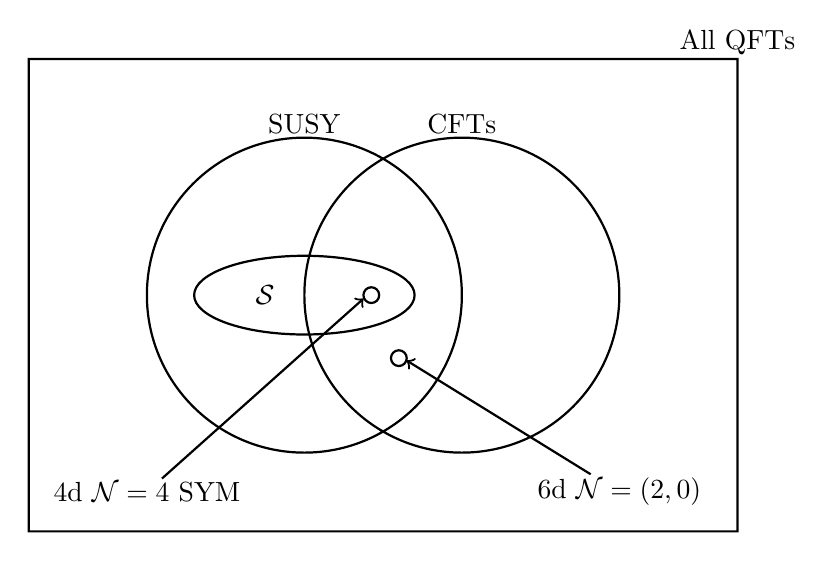
\begin{tikzpicture}[fill=white,thick,inner sep=0.1em]
% left hand
\scope
\clip (-4,-3) rectangle (4,3)
      (1.5,0) circle (2);
\fill (-0.5,0) circle (2);
\endscope
% right hand
\scope
\clip (-4,-3) rectangle (4,3)
      (-0.5,0) circle (2);
\fill (1.5,0) circle (2);
\endscope
% outline
\draw (-0.5,0) circle (2) (-0.5,2)  node [text=black,above] {SUSY}
      (1.5,0) circle (2) (1.5,2)  node [text=black,above] {CFTs}
      (-4,-3) rectangle (5,3) node [text=black,above] {All QFTs};
     \draw (-0.5,0) ellipse (1.4cm and 0.5cm);
     \node at (-1,0) {$\mathcal{S}$};
      \draw (0.35,0) circle (0.1) node (a)[below,left]{};
      \node (b) at (-2.5,-2.5) {4d $\mathcal{N}=4$ SYM};
      \draw [->] (b) to (a);
            \draw (0.7,-0.8) circle (0.1) node (c)[below,right]{};
      \node (d) at (3.5,-2.5) {6d $\mathcal{N}=(2,0)$};
      \draw [->] (d) to (c);
\end{tikzpicture}
  \caption{\it Schematic overview of the `landscape' of quantum field theories.}
  \label{fig:lndscpeofqfts}
\end{figure}

A more ambitious goal that has been initiated is to classify/construct all possible four dimensional $\mathcal{N}=2$ theories \cite{Argyres:2016xua,Argyres:2015gha,Bhardwaj:2013qia,KOH1984397,DERENDINGER1984133,JIANG1984370,Jiang_1984}.

\subsection{Class \texorpdfstring{$\mathcal{S}$}{S}}
A particularly useful tool to construct a large class of 4d $\mathcal{N}=2$ theories has been via compatification of the 6d $\mathcal{N}=(2,0)$ theories \cite{Gaiotto:2009we,Gaiotto:2009hg}.  We discussed these theories in Section \ref{eqn:introS1xMd} of this chapter.  Again we focus on the theories of $A_{N-1}$ type; realised as the worldvolume theory of a stack of $N$ parallel and coincident M$5$-branes.  

The 4d $\mathcal{N}=2$ theories engineered by compactifying this theory on a Riemann surface $\mathcal{C}$ are said to be of `class $\mathcal{S}$'.  Note that in order to preserve supersymmetry we must partially twist the $(2,0)$ theory.  This is achieved as follows.  The superconformal algebra is \cite{Kac:1977qb,Nahm:1977tg}
\begin{equation}
\mathfrak{osp}(8^*|4)\supset\mathfrak{so}(6)\oplus\mathfrak{so}(5)_R\,,
\end{equation}
in particular, the supercharges $\Qsix$ transform in the $(\mathbf{4},\mathbf{4})$ representation of the subalgebra.  Because we put the 6d theory on a product manifold $\mathbb{R}^4\times \mathcal{C}$ we decompose $\mathfrak{so}(6)\supset\mathfrak{so}(4)\oplus \mathfrak{u}(1)_s$.  For the purposes of the twisting we also decompose $\mathfrak{so}(5)_R\supset\mathfrak{su}(2)_R\oplus\mathfrak{u}(1)_r$.  Under the decomposition $\mathfrak{so}(4)\oplus \mathfrak{u}(1)_s\oplus\mathfrak{su}(2)_R\oplus\mathfrak{u}(1)_r$ the supercharges transform as
\begin{equation}
\Qsix\in(\mathbf{2},\frac{1}{2},\mathbf{2},\frac{1}{2})\oplus(\mathbf{2},\frac{1}{2},\overline{\mathbf{2}},-\frac{1}{2})\oplus(\overline{\mathbf{2}},-\frac{1}{2},\mathbf{2},\frac{1}{2})\oplus(\overline{\mathbf{2}},-\frac{1}{2},\overline{\mathbf{2}},-\frac{1}{2})\,.
\end{equation}
The twisting procedure then involves replacing the holonomy algebra with the diagonal subgroup $\mathfrak{u}(1)_s\to \mathfrak{u}(1)_{s'}\subset\mathfrak{u}(1)_r\oplus \mathfrak{u}(1)_s$.  After the twisting, under $\mathfrak{so}(4)\oplus\mathfrak{su}(2)_R\oplus\mathfrak{u}(1)_{r}\oplus\mathfrak{u}(1)_{s'}$,
\begin{equation}
\Qsix\in(\mathbf{2},\mathbf{2},1,\frac{1}{2})\oplus(\mathbf{2},\overline{\mathbf{2}},0,-\frac{1}{2})\oplus(\overline{\mathbf{2}},\mathbf{2},0,\frac{1}{2})\oplus(\overline{\mathbf{2}},\overline{\mathbf{2}},-1,-\frac{1}{2})\,,
\end{equation}
in particular we identify the eight $\mathfrak{u}(1)_{s'}$ scalar supercharges with the $\mathcal{N}=2$ supercharges.  Therefore, protected quantities of the 4d theory are independent of the choice of metric on $\mathcal{C}$ and depend only on the complex structure moduli.  More rigorously, the space of UV gauge couplings is identified with the space of complex structure deformations $\mathcal{E}$ of the underlying surface $\mathcal{C}$.  We have an isomorphism 
\begin{equation}
\mathcal{E}\iso Teich(\mathcal{C})/ MCG(\mathcal{C})
\end{equation}
where $Teich(\mathcal{C})$ is the Teichm\"uller space of $\mathcal{C}$ and is parametrised by the same cross ratios $q$ appearing in the Seiberg-Witten curve.  $MCG(\mathcal{C})$ is the mapping class group of $\mathcal{C}$, in physics terms this is the `generalised S-duality group'.  Moreover, the Seiberg-Witten curve for the class $\mathcal{S}$ theory is then obtained as a $\rank \mathfrak{g}$ cover of the underlying Riemann surface $\mathcal{X}_u\xrightarrow[]{\rank \mathfrak{g}:1}\mathcal{C}$.
In addition, many protected quantities, such as partition functions and correlation functions of BPS operators, in class $\mathcal{S}$ SCFTs may be computed as observables of a 2d theory which lives on $\mathcal{C}$ \cite{Alday:2009aq,Alday:2009fs}.  One manifestation of this 4d/2d relation is that the partition function on an ellipsoid $\mathbb{S}^4_{\epsilon_1,\epsilon_2}$ \eqref{eqn:introS4part} is equal to correlators in Liouville/Toda CFT \cite{Alday:2009aq,Wyllard:2009hg}.  In particular, the 2d Virasoro/W-algebra conformal blocks are mapped to Nekrasov's instanton partition function.  Another manifestation of a 4d/2d relation is the partition function on $\mathbb{S}^3\times \mathbb{S}^1$ \eqref{eqn:S1Mdm1part} which can be recast as a correlator of a 2d TQFT living on $\mathcal{C}$ \cite{Gadde:2009kb,Gadde:2011ik}.

Using the above compactification procedure we can generate an infinite number of 4d $\mathcal{N}=2$ theories labelled by compact Riemann surfaces $\mathcal{C}$.  These Riemann surfaces also carry marked punctured, corresponding to inserting a variety (while still preserving eight supercharges) of defect operators of the 6d theory at the punctures.

For the case of $\mathfrak{g}=A_{N-1}$ these $\frac{1}{2}$-BPS defect operators are labelled by Young tableaux \cite{Gaiotto:2009hg,Gaiotto:2009we} with $N$ boxes.  The two main punctures that we will discuss are `maximal' punctures labelled by tableaux of type $N=1+1+\dots+1$ and `minimal' punctures of type $N=(N-1)+1$.

For example, the $\mathcal{N}=2$ hypermultiplet is obtained by compactification of the $(2,0)$ theory on a sphere with a minimal puncture and two maximal punctures, this is pictured in Figure \ref{fig:n2hypersclassS}.
\begin{figure}
\centering
\begin{tikzpicture}[square/.style={regular polygon,regular polygon sides=4},thick,scale=0.8]
  \node(FR) at (2,0)[square,draw]{$N$};
  \node(FL) at (-1,0)[square,draw]{$N$};
  \node (eq) at (3.5,0) {$=$};
  \draw (FR)--(FL);
  \draw (6.5,0) ellipse (2.3cm and 1.7cm);
  \node at (5.5,-0.5) {\tiny $\yng(2)\dots\yng(1)$};
  \node at (7.5,-0.5) {\tiny $\yng(2)\dots\yng(1)$};
  \draw [black,fill=black] (6.5,0.75) circle (2pt);
\end{tikzpicture}
\caption{\textit{$\mathcal{N}=2$ hypermultiplets in the class $\mathcal{S}$ description.  The dot represents the $N=(N-1)+1$ minimal puncture.}}
\label{fig:n2hypersclassS}
\end{figure}
From this basic building block we can construct linear and affine quivers with $n$ gauge nodes, corresponding to spheres with $n+1$ minimal plus two maximal punctures and tori with $n$ minimal punctures, respectively.
For example, conformal $\mathcal{N}=2$ $N_f=2N$ SQCD can be made by gluing two of these three-punctured spheres together with a tube connecting the punctures, interpreted as gauging the flavour symmetry.  This is pictured in Figure \ref{fig:n2SCQCDsclassS}.  The punctures can be mapped, via conformal transformation, to $z=0,1,q,\infty$ and $q$ is identified with the complexified gauge coupling via $q=e^{2\pi\iu\tau_{\text{YM}}}$.
\begin{figure}
\centering
\begin{tikzpicture}[square/.style={regular polygon,regular polygon sides=4},thick,scale=0.8]
  \node(G) at (0,0)[circle,draw]{$N$};
  \node(FR) at (2,0)[square,draw]{$N$};
  \node(FL) at (-2,0)[square,draw]{$N$};
  \node (eq) at (3,0) {$=$};
  \draw (FR)--(G);
  \draw (FL)--(G);
  \draw (6.5,0) ellipse (2.6cm and 1.7cm);
  \node [label=below:{\tiny $0$}]at (5,-0.5) {\tiny $\yng(2)\dots\yng(1)$};
  \node [label=below:{\tiny $\infty$}] at (8,-0.5) {\tiny $\yng(2)\dots\yng(1)$};
    \draw [black,fill=black] (5.5,0.75) circle (2pt) node[below]{\tiny $1$};
   \draw[black,fill=black] (7.5,0.75) circle (2pt) node[below]{\tiny $q$};
\end{tikzpicture}
\caption{\textit{$\mathcal{N}=2$ SQCD with $N_f=2N$ hypermultiplets in the class $\mathcal{S}$ description.}}
\label{fig:n2SCQCDsclassS}
\end{figure}
 
Within this class the majority of theories do not admit known Lagrangian descriptions.  Indeed, with generic defect operators inserted, any other type of description of the resulting 4d theory is often lacking.  
Examples of non-Lagrangian theories that may be engineered within class $\mathcal{S}$ are the so-called $T_N$ SCFTs \cite{Gaiotto:2009we}.  These correspond to spheres with three maximal punctures.  For example, the $T_3$ theory.  This theory is the same as the rank one $E_6$ SCFT of Minihan and Nemeschansky \cite{Minahan:1996fg}, $T_3=MN(E_6)$.  To find this SCFT we begin with the $N=3$, $N_f=2N=6$ superconformal QCD, described in Figure \ref{fig:n2SCQCDsclassS}.  According to Argyres-Seiberg duality  \cite{Argyres:2007cn} in the $\tau_{\text{YM}}\to1$ region of this theory it admits a dual description in terms of the $MN(E_6)$ SCFT weakly coupled to a single $SU(2)$ hypermultiplet.  This is neatly illustrated within class $\mathcal{S}$ as we begin with the four punctured sphere and consider the limit where we collide the two minimal punctures at $z=1,q$ together, see Figure \ref{fig:T3sclassS}.
\begin{figure}
\centering
\begin{tikzpicture}[square/.style={regular polygon,regular polygon sides=4},thick,scale=0.8]
  \node(G) at (0,0)[circle,draw]{$3$};
  \node(FR) at (2,0)[square,draw]{$3$};
  \node(FL) at (-2,0)[square,draw]{$3$};
  \node (eq) at (3,0) {$=$};
   \node [label=below:$\Big\downarrow$] at (3,-2) {$q\to 1$};
  \draw (FR)--(G);
  \draw (FL)--(G);
  \draw (6.5,0) ellipse (2.5cm and 1.7cm);
  \node [label=below:{\tiny $0$}]at (5,-0.5) {\tiny $\yng(3)$};
  \node [label=below:{\tiny $\infty$}] at (8,-0.5) {\tiny $\yng(3)$};
  \draw [black,fill=black] (5.5,0.75) circle (2pt) node[below]{\tiny $z=1$};
   \draw[black,fill=black] (7.5,0.75) circle (2pt) node[below]{\tiny $z=q$};
   \node(G1) at (0,-4)[circle,draw]{$2$};
  \node(FR1) at (2,-4)[square,draw]{$1$};
  \node(T3) at (-1.5,-4)[circle,draw]{$T_3$};
  \node at (-0.75,-4) {$\subset$};
  \node (eq) at (3,-4) {$=$};
  \draw (FR1)--(G1);
    \draw (6.5,-4) ellipse (2.5cm and 1.7cm);
  \node [label=below:{\tiny $0$}]at (5,-4.5) {\tiny $\yng(3)$};
  \node (gau) [label=below:{\tiny $1$}] at (8,-4.5) {\tiny $\yng(3)$};
  \node [label=below:{\tiny $\infty$}] at (6.5,-3.25) {\tiny $\yng(3)$};
  \draw (11.5,-4) ellipse (2cm and 1.3cm);
  \draw [black,fill=black] (12.5,-4.5) circle (2pt);
   \draw[black,fill=black] (12,-3.5) circle (2pt);
   \draw (gau.north) to[bend right=5] (11, -4.4);
   \draw (gau.south) to[bend left=5] (11, -4.6);
\end{tikzpicture}
\caption{\textit{Description of the $T_3=MN(E_6)$ SCFT in class $\mathcal{S}$ description.}}
\label{fig:T3sclassS}
\end{figure} 
These types of manipulations may be used to also find the class $\mathcal{S}$ descriptions of the $MN(E_7)$ \& $MN(E_8)$ SCFTs \cite{Minahan:1996cj}.  Moreover, applying the same logic new strong-weak dual descriptions are able to be conjectured, see e.g.  \cite{Tachikawa:2013kta} for more information on these points.

\subsection{Class \texorpdfstring{$\mathcal{S}_k$}{Sk}}\label{sec:introSk}
$\mathcal{N}=1$ variations of the class $\mathcal{S}$ construction have been proposed in \cite{Gaiotto:2015usa,Bah:2017gph,Heckman:2016xdl,Razamat:2016dpl,Coman:2015bqq,Morrison:2016nrt,Franco:2015jna,Hanany:2015pfa,Apruzzi:2016nfr,DelZotto:2017pti,Apruzzi:2017iqe,Hassler:2017arf,Kim:2018lfo,Razamat:2018gro}.  
The idea is to obtain 4d $\N=1$ theories via (twisted) compactification of 6d $(1,0)$ SCFTs again on punctured Riemann surfaces $\mathcal{C}$.  $\frac{1}{2}$-BPS defect operators of the $(1,0)$ theory can then be localised at the punctures on $\mathcal{C}$ to create a wide variety of $\mathcal{N}=1$ theories.  

The landscape of 6d $(1,0)$ SCFTs is far richer than that of $(2,0)$ theories; in addition to their respective superconformal symmetries $(2,0)$ theories can have only discrete global symmetries while $(1,0)$ theories can also have continuous flavour symmetry groups (this is analagous to the difference in the possible 4d $\mathcal{N}=4$ versus $\mathcal{N}=2$ theories).  An F-theoretic classification of $(1,0)$ theories has been explored in \cite{Heckman:2013pva,DelZotto:2014hpa,Heckman:2015bfa,Bhardwaj:2015oru} but a complete field theoretic understanding is currently lacking.  

Let us outline the twisting procedure for the $(1,0)$ theories.  The R-symmetry is now $\mathfrak{su}(2)$ under which the supercharges are in the fundamental representation and again in the spinor represenation of $\mathfrak{so}(6)$.  In this case one chooses a $\mathfrak{so}(4)\oplus\mathfrak{u}(1)_s\subset\mathfrak{so}(6)$ and $\mathfrak{u}(1)_{r'}\subset\mathfrak{su}(2)_R$.  Under $\mathfrak{so}(4)\oplus\mathfrak{u}(1)_s\oplus\mathfrak{u}(1)_{r'}$
\begin{equation}\label{eqn:Sktopotwist}
\Qsix\in(\mathbf{2},\frac{1}{2},\frac{1}{2})\oplus(\mathbf{2},\frac{1}{2},-\frac{1}{2})\oplus(\overline{\mathbf{2}},-\frac{1}{2},\frac{1}{2})\oplus(\overline{\mathbf{2}},-\frac{1}{2},-\frac{1}{2})\,.
\end{equation}
Now replacing $\mathfrak{u}(1)_s\to \mathfrak{u}(1)_{s'}\subset\mathfrak{u}(1)_{r'}\oplus \mathfrak{u}(1)_s$ we have four $\mathfrak{u}(1)_{s'}$-scalar supercharges which are identified with the supercharges of the 4d $\mathcal{N}=1$ superalgebra.

An interesting subset of 6d $(1,0)$ theories are those which may be engineered within M-theory by considering the low energy theory living on $N$ coincident and parallel M$5$-branes at the tip of a transverse $\Gamma=ADE$ singularity.  These $(1,0)$ theories are orbifolds of the $\mathfrak{g}=A_{N-1}$ $(2,0)$ theory, which we denote by $(1,0)_{\Gamma}$.  4d $\mathcal{N}=1$ theories obtained in this way are said to lie within `class $\mathcal{S}_{\Gamma}$' \cite{Gaiotto:2015usa,Heckman:2016xdl}.  The 4d theories of type $\Gamma=A_{k-1}$ will be one of the primary subjects of this thesis; theories of this type will be designated to be that of `class $\mathcal{S}_{k}$'.

In contrast to the $(2,0)$ theories (who's $\frac{1}{2}$-BPS defect operators are simply classified by Young's tableaux) the permissible defect operators for the $(1,0)_{\Gamma}$ theories have a very complicated classification \cite{Heckman:2016xdl}.  Moreover, descriptions of the resulting 4d $\mathcal{N}=1$ theories upon compactification are currently lacking for all but a few configurations of punctures.

In \cite{Gaiotto:2015usa} the superconformal index was computed for a variety of class $\mathcal{S}_k$ theories and most strikingly it was recast as a correlator of a 2d TQFT establishing the first 2d/4d relation for class $\mathcal{S}_k$.  Subsequently, in \cite{Ito:2016fpl,Maruyoshi:2016caf}, the index and its TQFT description was also computed in the presence of $\frac{1}{2}$-BPS surface defects.  Additionally, in \cite{Coman:2015bqq}, SW curves were computed and some of their properties explored.  In \cite{Mitev:2017jqj}, guided by the SW curves, the existence of an AGT-like correspondence for the class $\mathcal{S}_k$, denoted AGT$_k$ correspondence, was conjectured.  Furthermore, the instanton partition function was proposed  via a relation to $\mathcal{W}_{kN}$ conformal blocks.
\subsubsection{4d $\mathcal{N}=1$ Class $\mathcal{S}_k$ Quiver Gauge Theories}\label{sec:quivers}
In this section we review some basic details of the `core theories' in class $\mathcal{S}_k$ introduced in \cite{Gaiotto:2015usa}.  We will mostly follow the notation of \cite{Razamat:2018zus}.

As we have discussed, we realise the theories in the class $\mathcal{S}_k$ as twisted compactifications along a Riemann surface of genus $g$ with $\ell$ punctures of the $(1,0)_{A_{k-1}}$ SCFT.  The 6d theory has a $\mathfrak{u}(1)_t\oplus\mathfrak{su}(k)_{\beta}\oplus\mathfrak{su}(k)_{\gamma}$ global symmetry.  The compactifications typically preserve only a Cartan subalgebra $\mathfrak{u}(1)_t\oplus\mathfrak{u}(1)^{\oplus k-1}_{\beta}\oplus\mathfrak{u}(1)^{\oplus k-1}_{\gamma}$ which are `intrinsic' global symmetries carried by all class $\mathcal{S}_k$ theories.  There is also the $\mathcal{N}=1$ $\mathfrak{u}(1)_r$ R-symmetry.
The punctures carry additional data associated to inserting a variety of defect operators localised at the punctures in six dimensions \cite{Gaiotto:2015usa,Hassler:2017arf,Heckman:2016xdl}, in this paper we will focus only on maximal and minimal punctures.  

Maximal punctures are labelled with a colour $c\in \{1,2,\dots,k\}$, a sign $\sigma=\pm1$ and an orientation $o=l/r$.  We will label these maximal punctures with the notation $s_{c}^{o,\sigma}$.  Maximal punctures also carry an associated $\mathfrak{su}(N)^{\oplus k}$ flavour symmetry algebra.  Minimal punctures carry a $\mathfrak{u}(1)$ symmetry under which the baryonic operators of the form $\det Q_i$, $\det \widetilde{Q}_i$ and $\det\Phi_i$ are charged while mesonic operators are uncharged.

The core theories that we will focus on are associated to spheres with $\ell-2$ minimal punctures and two maximal punctures $s_{c_l}^{l,+}$ \& $s_{c_r}^{r,+}$  with $c_r=(c_l+\ell-2)\bmod k$, and $\frac{1}{2k}$ unit of flux for $U(1)_t$.  These admit a quiver description, as shown in FIgure \ref{fig:Skquivergenus0}.

This theory admits a weakly coupled Lagrangian description associated to a pair of pants decomposition of the Riemann surface into a chain of $n=0,1,\dots,\ell-3$ spheres with one minimal puncture and two maximal punctures $s_{c_l+n}^{l,+}$ \& $s_{c_l+n+1}^{r,+}$.  These three punctured spheres correspond to quiver theories of bifundamental chiral multiplets called the \textit{free trinion} and is pictured in Figure \ref{fig:freetrinion}.
\begin{figure}
\centering
\begin{subfigure}{.5\textwidth}
\centering
\begin{tikzpicture}[square/.style={regular polygon,regular polygon sides=4},thick,inner sep=0.1em,scale=0.7]
    %gaugenodes  
    \node (L1) at (0,0) [square,draw,minimum size=1.8cm]{$i-1$};
    \node (R1) at (4,0) [square,draw,minimum size=1.8cm]{$i-1$};
    \node (L2) at (0,-3) [square,draw,minimum size=1.8cm]{$i$};
    \node (R2) at (4,-3) [square,draw,minimum size=1.8cm]{$i$};
    \node (L3) at (0,-6) [square,draw,minimum size=1.8cm]{$i+1$};
    \node (R3) at (4,-6) [square,draw,minimum size=1.8cm]{$i+1$};

    \draw [->] (L1.0) -- (R1.180) node[midway,above] {$Q_{i-1}$};
    \draw [->] (L2.0) -- (R2.180) node[midway,above] {$Q_{i}$};
    \draw [->] (L3.0) -- (R3.180) node[midway,above] {$Q_{i+1}$};
    
    \draw [->] (R1.225) -- (L2.45) node[midway,above,sloped] {$\widetilde{Q}_{i}$};
    \draw [->] (R2.225) -- (L3.45) node[midway,above,sloped] {$\widetilde{Q}_{i+1}$};
     \draw  (R3.225) -- (2,-7.5) node[near end,above,sloped] {$\widetilde{Q}_{i+2}$};
      \draw [->] (2,1.5) -- (L1.45) node[near start,above,sloped] {$\widetilde{Q}_{i-1}$};
     
 \end{tikzpicture}
 \end{subfigure}%
 \begin{subfigure}{.5\textwidth}
 \centering
  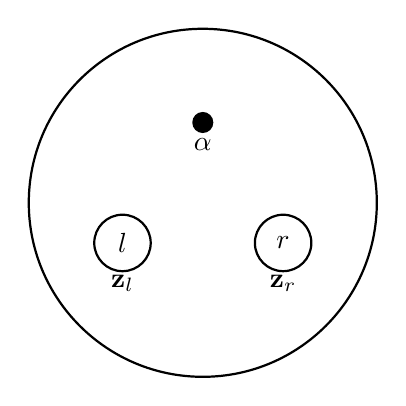
\begin{tikzpicture}[thick,scale=1.7]
  \draw (0,0) ellipse (1.3cm and 1.3cm);
  \draw [black,fill=black] (0,0.6) circle (2pt) node [below=2pt]{$\alpha$};
  \draw [black] (-0.6,-0.3) circle (6pt) node [below=8pt]{$\mathbf{z}_l$} node{$l$};
  \draw [black] (0.6,-0.3) circle (6pt) node [below=8pt]{$\mathbf{z}_r$} node {$r$};

\end{tikzpicture}
 \end{subfigure}%
  \caption{\it Quiver diagram for the free trinion theory of bifundamental chiral multiplets, associated to a sphere with one minimal puncture and two maximal punctures $s_{c}^{l,+}$ and $s_{c+1}^{r,+}$.}
  \label{fig:freetrinion}
\end{figure}
The maximal punctures of equal colour, opposite orientation and equal sign of the $n^{\text{th}}$ and $(n+1)^{\text{th}}$ three punctured spheres are then glued with tubes associated to spheres with two maximal punctures $s_{c_l+n+1}^{l,+}$ \& $s_{c_l+n+1}^{r,+}$.  This gluing corresponds to gauging the diagonal $\mathfrak{su}(N)_{\mathbf{z}}^{\oplus k}\subset\mathfrak{su}(N)_{\mathbf{z}_l}^{\oplus k}\oplus \mathfrak{su}(N)_{\mathbf{z}_r}^{\oplus k}$ of the two maximal punctures with free $\mathcal{N}=1$ vector multiplets and $k$ bifundamental chiral multiplets $\Phi_i$.
This type of gluing is called $\Phi$-gluing and is pictured in Figure \ref{fig:tube}.  This leads to quiver theories of the type pictured in Figure \ref{fig:Skquivergenus0}.  The representations of the fields under the global symmetries are summarised in Table \ref{tab:lettersphi} and will be used later.  

From these theories it is possible to construct theories associated to tori with $\ell-2$ minimal punctures by $\Phi$-gluing the `open' maximal punctures $s_{c_l}^{l,+}$ \& $s_{c_r}^{r,+}$, these are $\mathbb{Z}_k\times\mathbb{Z}_{\ell-2}$ orbifold theories of $\mathcal{N}=4$ SYM.  Unless $c_r-c_l=0\bmod k$ (or equivilantly $\ell-2\bmod k=0$) this procedure breaks the $\mathfrak{u}(1)^{\oplus k-1}_{\beta}\oplus\mathfrak{u}(1)^{\oplus k-1}_{\gamma}$ symmetry.  The quiver diagram of such theories can be found in Figure \ref{fig:Skquivergenus1}.  This leads to quiver theories of this type shown in Figure \ref{fig:Skquivergenus1}.
\begin{figure}
\centering
\begin{subfigure}{.5\textwidth}
\centering
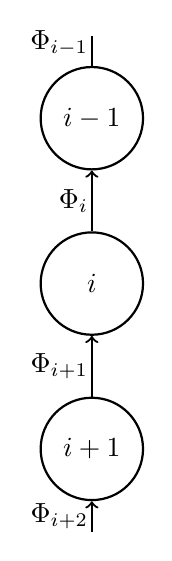
\begin{tikzpicture}[thick,inner sep=0.1em,scale=0.7]
    %gaugenodes  
    \node (L1) at (0,0) [circle,draw,minimum size=1.3cm]{$i-1$};
    \node (L2) at (0,-3) [circle,draw,minimum size=1.3cm]{$i$};
    \node (L3) at (0,-6) [circle,draw,minimum size=1.3cm]{$i+1$};
    
    \draw [->] (0,-7.5) -- (L3.270) node[near start,midway,left] {$\Phi_{i+2}$};    
    \draw [->] (L3.90) -- (L2.270) node[midway,left] {$\Phi_{i+1}$};
    \draw [->] (L2.90) -- (L1.270) node[midway,left] {$\Phi_{i}$};
    \draw [-] (L1.90) -- (0,1.5) node[near end,left] {$\Phi_{i-1}$};
     
 \end{tikzpicture}
 \end{subfigure}%
 \begin{subfigure}{.5\textwidth}
 \centering
  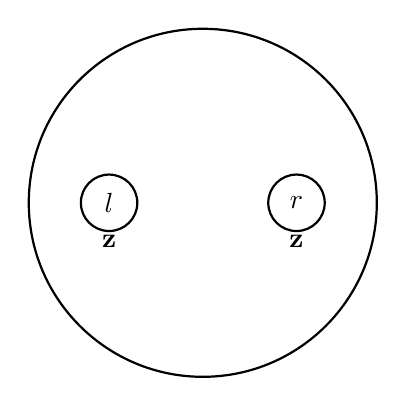
\begin{tikzpicture}[thick,scale=1.7]
  \draw (0,0) ellipse (1.3cm and 1.3cm);
  \draw [black] (-0.7,0) circle (6pt) node [below=8pt]{$\mathbf{z}$} node{$l$};
  \draw [black] (0.7,0) circle (6pt) node [below=8pt]{$\mathbf{z}$} node {$r$};

\end{tikzpicture}
 \end{subfigure}%
  \caption{\it Quiver associated to $\Phi$-gluing.}
  \label{fig:tube}
\end{figure}

Finally, a general Lagrangian theory in class $\mathcal{S}_k$, made using the above ingredients, associated to a genus $g$ Riemann surface with $\ell$ punctures has superpotential
\begin{equation}\label{eqn:Sksuperpotential}
\begin{aligned}
W_{\mathcal{S}_k}=&\sum_{n=1}^{3g-3+\ell}\sum_{i=1}^k\tr\left( \widetilde{Q}_{(i,n-1)}Q_{(i,n-1)}\Phi_{(i,n)}-Q_{(i-1,n)}\widetilde{Q}_{(i,n)}\Phi_{(i,n)}\right)\\
&+\sum_{n=1}^{3g-3+\ell}\sum_{i=1}^k\frac{\tau_{YM,ni }}{8\pi\iu}\tr W^{\alpha}_{ni}W_{ni,\alpha}\,.
\end{aligned}
\end{equation}
One may also generate other Lagrangian theories associated to spheres with one minimal puncture and two maximal puncture with a variety of different configurations $s_c^{o,\sigma}$ by, for example, turning on flux for $U(1)_t$.  We will not consider these theories in this thesis.
\subsubsection{Type-II Description}\label{sec:stringsetup}
In this section we present the brane setups which we use to `engineer' Lagrangian theories in class $\mathcal{S}_k$.
We begin with the toroidal $\N=1$ quiver theories in class $\mathcal{S}_k$  which are obtained using Type-IIB string theory with $N$ D3 branes probing a $\mathbb{Z}_\ell \times \mathbb{Z}_k$  orbifold singularity (Table \ref{table:D3D-1}).
They are examples of $\mathcal{N}=1$ orbifold daughters of $\mathcal{N}=4$ SYM \cite{Kachru:1998ys,Lawrence:1998ja} and were extensively studied in the early days of $AdS$/CFT.  After T-duality we land on Type-IIA string theory with $N$ D4 and $\ell$ NS5 branes in the presence of a $\mathbb{Z}_k$ orbifold singularity, which was used in \cite{Gaiotto:2015usa}, this is the Hanany-Witten picture.  From the Type-IIA setup we can consider a decoupling limit upon which we arrive at the 'core theories' corresponding to spheres with two maximal punctures and a collection of minimal punctures.
\paragraph{Type-IIB}
Consider Type-IIB string theory on $\mathbb{R}^4\times\mathbb{R}^6/\Gamma$ with $\Gamma=\mathbb{Z}_{\ell}\times\mathbb{Z}_k$ with $\ell,k\in\mathbb{Z}^+$.  Our goal is to engineer the class $\mathcal{S}_k$ theories corresponding to a torus with $\ell$ minimal punctures within Type-IIB string theory.  Hence, we add a set of $N$ parallel and coincident D$3$ branes along the $\mathbb{R}^4$ as described in Table \ref{table:D3D-1}.  We parametrise the worldvolume of the D$3$ branes with four real coordinates $X^1,X^2,X^3,X^4$, which arrange themselves into the vector representation of $Spin(4)\iso SU(2)_{\alpha}\times SU(2)_{\dot\alpha}$.  The Cartans $j_1,j_2$, of $\mathfrak{su}(2)_{\alpha},\mathfrak{su}(2)_{\dot\alpha}$ are defined such that lower $\alpha=1,2$ have $j_1=+\frac{1}{2},-\frac{1}{2}$ and $\dot{\alpha}=\dot1,\dot2$ have $j_2=+\frac{1}{2},-\frac{1}{2}$.  The $\mathbb{R}^6\iso\mathbb{C}^3$ is parametrised by six real coordinates $X^5,X^6,X^7,X^8,X^9,X^{10}$ and the isomorphism is made by the choice of arrangement into the complex coordinates
\begin{gather}
\label{eqn:coordinates}
%\Phi^1 
z_1
:=\frac{X^5+\iu X^6}{\sqrt{2}}=\Phi|_{\theta=0},\quad 
%Phi^2 
z_{2}
:=\frac{X^7+\iu X^{10}}{\sqrt{2}}=Q|_{\theta=0},\quad 
%\Phi^3 
\\
z_3
:=\frac{X^8+\iu X^9}{\sqrt{2}}=\widetilde{Q}|_{\theta=0}
\end{gather} 
and their hermitian conjugates.
\begin{table}
\centering
\begin{tabular}{ |c |c| c| c| c| c| c| c| c| c| c| }
\hline
   & $X^1$ & $X^2$ & $X^3$ & $X^4$ & $X^5$ & $X^6$ & $X^7$ & $X^8$ & $X^9$& $X^{10}$\\\hline 
 $N$ D$3$ & -- & -- & -- & -- & $\cdot$ & $\cdot$ & $\cdot$ & $\cdot$ & $\cdot$ & $\cdot$\\ \hline
 $A_{\ell-1}$ & $\cdot$ & $\cdot$ & $\cdot$ & $\cdot$ & $\cdot$ & $\cdot$ & $\times$ & $\times$ & $\times$ & $\times$\\ \hline
 $A_{k-1}$ & $\cdot$ & $\cdot$ & $\cdot$ & $\cdot$ & $\times$ & $\times$ & $\cdot$ & $\times$ & $\times$ & $\cdot$\\ \hline
\end{tabular}
\caption{\it Type-IIB setup engineering Lagrangian 4d SCFTs in class $\mathcal{S}_k$.}
\label{table:D3D-1}
\end{table}
The orbifold $\Gamma$ acts on those coordinates \eqref{eqn:coordinates} as
\begin{equation}\label{eqn:orbifoldactionR10}
(z_1,z_2,z_3)\mapsto(\omega_kz_1,\omega_{\ell}z_2,\omega_{\ell}^{-1}\omega^{-1}_{k}z_3)\,,\quad \omega_k^k=\omega_{\ell}^{\ell}=1\,.
\end{equation}
Before the orbifold action, fundamental strings stretching between D$3$ branes give rise to the $SU(N)$ $\N=4$ SYM theory on their worldvolume; with $R$-symmetry $Spin(6)_R\iso SU(4)_R$, the rotation group of the transverse $\mathbb{R}^6$.  In $\N=1$ superspace the theory contains a vector multiplet $\mathcal{V}$ and three chiral superfields in the adjoint of the gauge group: $\left(\Phi,Q,\widetilde{Q}\right)$ transforming in the $\mathbf{3}$ of $SU(3)_R\subset SU(4)_R$.  The superpotential is given by
\begin{equation}
W_{\N=4}=\tr\Phi[Q,\widetilde{Q}]+\frac{\tau_{YM}}{8\pi\iu}\tr W^{\alpha}W_{\alpha}\,.
\end{equation}
The chiral superfields are identified with transverse coordinates \eqref{eqn:coordinates} hence the action of $\Gamma$ on $\mathbb{C}^3$ lies diagonally inside $SU(3)_{R}$ in the form
\begin{equation}
M:=\begin{pmatrix}
\omega_k&0&0\\
0&\omega_{\ell}&0\\
0&0&\omega_{\ell}^{-1}\omega_{k}^{-1}
\end{pmatrix}\in SU(3)_{R}\,.
\end{equation}
Note that $\Gamma$ also has an action inside the gauge group, $SU(N)$ \cite{Douglas:1996sw}.  Its action can be conjugated to an element $h$ of the maximal torus $T(SU(N))=U(1)^{N-1}$.  After scaling $N\to|\Gamma|N=\ell kN$ this action breaks $G\to \prod_{n=1}^{\ell}\prod_{i=1}^kSU(N_{ni})$ specified by a partition of $\ell kN=\sum_{n,i}N_{ni}$ into $\ell k$ integers.  Note we always take the orbifold indices to be $n,m=1,\dots,\ell$ and $i,j=1,\dots,k$ and we impose orbifold periodicity $n\sim n+\ell$, $i\sim i+k$.  To obtain the correct SCFT in class $\mathcal{S}_k$; we choose the action of $\Gamma$ such that $N_{ni}=N$ for all $n,i$.  Hence $h$ may be written as
\begin{equation}\label{eqn:orbifoldactionSUN}
h=\diag\left(\omega_{\ell}\omega^{-1}_k\mathbb{I},\dots,\omega_{\ell}\omega_k^{-k}\mathbb{I},\dots,\omega^{\ell}_{\ell}\omega_k^{-1}\mathbb{I},\dots, \omega_{\ell}^{\ell}\omega^{-k}_k\mathbb{I}\right)
\end{equation}
where $\mathbb{I}$ denotes the $N\times N$ identity matrix.  Quotienting by $\Gamma$ imposes the identifications
\begin{equation}
\mathcal{V}\sim h^{\dagger}\mathcal{V}h\,,\quad \begin{pmatrix}\Phi\\Q\\\widetilde{Q}\end{pmatrix}\sim M\begin{pmatrix}h^{\dagger}\Phi h\\h^{\dagger}Qh\\h^{\dagger}\widetilde{Q}h\end{pmatrix}\,.
\end{equation}
After performing these identifications the resulting theory is an $\N=1$ torodial quiver gauge theory with gauge group $SU\left(N\right)^{\ell k}$ and superpotential given by \eqref{eqn:Sksuperpotential}.  The fields now transform as $\Phi_{(n,i)}\in (N_{ni},\overline{N}_{n(i-1)})$, $Q_{(n,i)}\in (N_{ni},\overline{N}_{(n+1)i})$ and $\widetilde{Q}_{(n,i)}\in (N_{n(i-1)},\overline{N}_{(n-1)i})$ under the gauge group $\prod_{n,i}SU(N_{ni})=SU\left(N\right)^{\ell k}$.  We summarise the field content in the quiver diagram of Figure \ref{fig:Skquivergenus1}.  Horizontal lines between node $(i,n)$ and $(i,n+1)$ denote $Q_{(i,n)}$ fields.  Vertical lines between node $(i,n)$ and $(i-1,n)$ denote $\Phi_{(i,n)}$ fields.  Diagonal lines between $(i-1,n+1)$ and $(i,n)$ denote $\widetilde{Q}_{(i,n)}$ fields.  See also Section \ref{sec:modulispace}.  The quiver should be periodically identified in both directions, such that it has the topology of a tessellation of the  torus.  The individual couplings for each gauge node $g_{YM,ni}^2$ are given by integration of a non-zero $B$-field flux over the two-cycles $C_{ni}$ of the space obtained by resolving the $\mathbb{C}^3/\Gamma$ singularities
\begin{equation}\label{eqn:Bfield}
\int_{C_{ni}}B=\frac{4\pi^2}{g^2_{YM,ni}}\,,\quad \sum_{n,i}\frac{1}{g_{YM,ni}^2}=\frac{1}{g^2_{YM}}\,.
\end{equation}
These are precisely the same class of $\N=1$ SCFTs which we expect to describe, at low energies, the 4d theory obtained by placing $N$ M$5$-branes at the tip of an $A_{k-1}$ singularity), compactified on $T^2$ with $\ell$ punctures and complex structure $\tau_{YM}=\frac{4\pi\iu}{g_{YM}^2}+  \frac{\theta}{2\pi}$ \cite{Gaiotto:2015usa}.   
\begin{figure}
\centering
  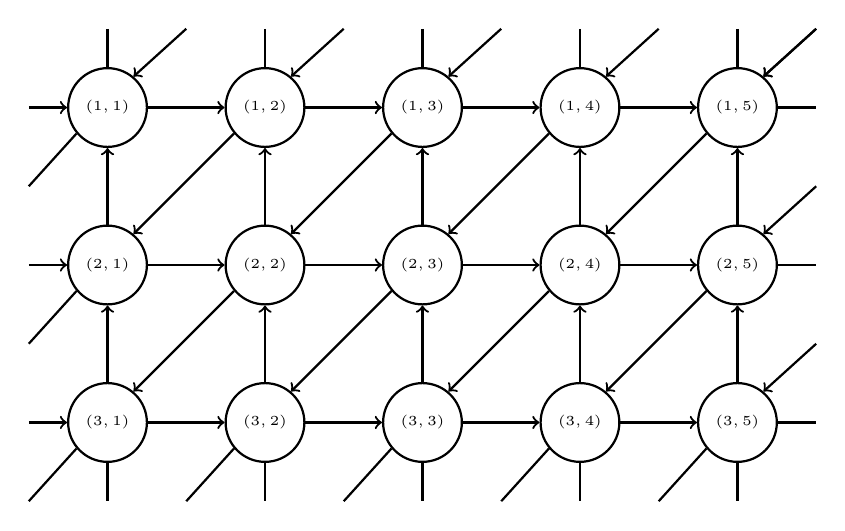
\begin{tikzpicture}[square/.style={regular polygon,regular polygon sides=4},thick,inner sep=0.1em,scale=1]
    %gaugenodes
    \node (G11) at (0,0)[circle,draw,minimum size=1cm]{\tiny $(1,1)$};
    \node (G21) at (2,0) [circle,draw,minimum size=1cm]{\tiny $(1,2)$};
    \node (G31) at (4,0) [circle,draw,minimum size=1cm]{\tiny $(1,3)$};
    \node (G41) at (6,0) [circle,draw,minimum size=1cm]{\tiny $(1,4)$};
    \node (G51) at (8,0)[circle,draw,minimum size=1cm]{\tiny $(1,5)$};
    \node (G12) at (0,-2)[circle,draw,minimum size=1cm]{\tiny $(2,1)$};
    \node (G22) at (2,-2) [circle,draw,minimum size=1cm]{\tiny $(2,2)$};
    \node (G32) at (4,-2) [circle,draw,minimum size=1cm]{\tiny $(2,3)$};
    \node (G42) at (6,-2)[circle,draw,minimum size=1cm]{\tiny $(2,4)$};
    \node (G52) at (8,-2)[circle,draw,minimum size=1cm]{\tiny $(2,5)$};
	\node (G13) at (0,-4)[circle,draw,minimum size=1cm]{\tiny $(3,1)$};
    \node (G23) at (2,-4) [circle,draw,minimum size=1cm]{\tiny $(3,2)$};
    \node (G33) at (4,-4) [circle,draw,minimum size=1cm]{\tiny $(3,3)$};
    \node (G43) at (6,-4)[circle,draw,minimum size=1cm]{\tiny $(3,4)$};
    \node (G53) at (8,-4)[circle,draw,minimum size=1cm]{\tiny $(3,5)$};
    
    %down chirals phi1
    \draw [<-] (G11.270) to (G12.90);
    \draw [<-] (G21.270) to (G22.90);
    \draw [<-] (G31.270) to (G32.90);
    \draw [<-] (G41.270) to (G42.90);
    \draw [<-] (G51.270) to (G52.90);
    \draw [<-] (G12.270) to (G13.90);
    \draw [<-] (G22.270) to (G23.90);
    \draw [<-] (G32.270) to (G33.90);
    \draw [<-] (G42.270) to (G43.90);
    \draw [<-] (G52.270) to (G53.90);
    \draw [-] (0,1) to (G11.90);
    \draw [-] (2,1) to (G21.90);
    \draw [-] (4,1) to (G31.90);
    \draw [-] (6,1) to (G41.90);
    \draw [-] (8,1) to (G51.90);
    \draw [-] (G13.270) to (0,-5);
    \draw [-] (G23.270) to (2,-5);
    \draw [-] (G33.270) to (4,-5);
    \draw [-] (G43.270) to (6,-5);
    \draw [-] (G53.270) to (8,-5);
    
    %right phi2
    \draw [->] (-1,0) to (G11.180);
    \draw [->](G11.0) to (G21.180);
    \draw [->] (G21.0) to (G31.180);
    \draw [->] (G31.0) to (G41.180);
    \draw [->] (G41.0) to (G51.180);
    \draw [-] (G51.0) to (9,0);
    \draw [->] (-1,-2) to (G12.180);
    \draw [->] (G12.0) to (G22.180);
    \draw [->] (G22.0) to (G32.180);
    \draw [->] (G32.0) to (G42.180);
    \draw [->] (G42.0) to (G52.180);
    \draw [-] (G52.0) to (9,-2);
    \draw [->] (-1,-4) to (G13.180);
    \draw [->] (G13.0) to (G23.180);
    \draw [->] (G23.0) to (G33.180);
    \draw [->] (G33.0) to (G43.180);
    \draw [->] (G43.0) to (G53.180);
    \draw [-] (G53.0) to (9,-4);
     
	
	%left up Phi3
    \draw [<-] (G11.50) to (1,1);
    \draw [<-] (G21.50) to (3,1);
    \draw [<-] (G31.50) to (5,1);
    \draw [<-] (G41.50) to (7,1);
    \draw [<-] (G51.50) to (9,1);

	\draw [<-] (G13.50) to (G22.220);
    \draw [<-] (G23.50) to (G32.220);
    \draw [<-] (G33.50) to (G42.220);
    \draw [<-] (G43.50) to (G52.220);
    \draw [<-] (G32.50) to (G41.220);
    \draw [<-] (G22.50) to (G31.220);
    \draw [<-] (G12.50) to (G21.220);
    \draw [<-] (G42.50) to (G51.220);
    
    \draw [-] (G13.220) to (-1,-5);
    \draw [-] (G12.220) to (-1,-3);
    \draw [-] (G11.220) to (-1,-1);
    \draw [-] (G23.220) to (1,-5);
    \draw [-] (G33.220) to (3,-5);
    \draw [-] (G43.220) to (5,-5);
    \draw [-] (G53.220) to (7,-5);
    \draw [<-] (G53.50) to (9,-3);
    \draw [<-] (G52.50) to (9,-1);
    \draw [<-] (G51.50) to (9,1);
    
  \end{tikzpicture}
  \caption{\it Section of the quiver diagram of the $\mathbb{Z}_k\times\mathbb{Z}_{\ell}$ orbifold theory of $\mathcal{N}=4$ SYM.  Circular nodes denote $(S)U(N)$ vector multiplets and directed arrows denote chiral multiplets.  }
  \label{fig:Skquivergenus1}
\end{figure}

\paragraph{Type-IIA}
By performing a T-duality along, say, $X^7$ to the setup of Table \ref{table:D3D-1} we may obtain the Hanany-Witten description of the above class $\mathcal{S}_k$ theories in Type-IIA as described in \cite{Gaiotto:2015usa}.  To perform the T-duality we may partially resolve the $\mathbb{C}^3/\Gamma$ singularity.  Resolving the $A_{\ell-1}$ singularity gives rise to an ALE space which is equivalent to the $\lambda\to\infty$ limit of the $\ell$-centred Taub-Nut space TN$_{\ell}$ with metric
\begin{equation}
ds^2=V^{-1}\left(d\Theta+\vec{A}\cdot d\vec{x}\right)^2+Vd\vec{x}^2,\quad V=\sum_{n=1}^{\ell}\frac{1}{\left|\vec{x}-\vec{x}_n\right|}+\frac{1}{\lambda^2}
\end{equation}
subject to the condition $\vec{\nabla}V=-\vec{\nabla}\times\vec{A}$.  The underlying geometry is that of an $\mathbb{S}^1$ fibered over an $\mathbb{R}^3$ base.  To perform the T-duality we hence replace $\mathbb{C}^3/\Gamma$ by $\left(\mathbb{C}\times \text{TN}_{\ell}\right)/\mathbb{Z}_{k}$ where $\mathbb{C}$ is parametrised by $z_{1},\overline{z}_{1}$ and TN$_{\ell}$ is parametrised by $\Theta=X^7$, $\vec{x}=\left(X^8,X^9,X^{10}\right)$.  We may then T-dualise along the TN$_{\ell}$ circle (which is invariant under the $\mathbb{Z}_{k}$ action).  We hence obtain the Hanany-Witten description shown in Table \ref{table:D4D01}.  Under the T-duality the $\ell$ centers of TN$_{\ell}$ become $\ell$ NS$5$-branes fixed at positions $\Theta_n$ and $\vec{x}_n$ in the transverse directions.
\begin{table}[h!]
\centering
\begin{tabular}{ |c |c| c| c| c| c| c| c| c| c| c| }
\hline
   & $X^1$ & $X^2$ & $X^3$ & $X^4$ & $X^5$ & $X^6$ & $X^7$ & $X^8$ & $X^9$& $X^{10}$\\\hline 
 $N$ D$4$ & -- & -- & -- & -- & $\cdot$ & $\cdot$ & -- & $\cdot$ & $\cdot$ & $\cdot$\\ \hline
 $\ell$ NS$5$ & -- & -- & -- & -- & -- & -- & $\cdot$ & $\cdot$& $\cdot$ & $\cdot$\\ \hline
 $A_{k-1}$ & $\cdot$ & $\cdot$ & $\cdot$ & $\cdot$ & $\times$ & $\times$ & $\cdot$ & $\times$ & $\times$ & $\cdot$\\ \hline
\end{tabular}
\caption{\it The Type-IIA setup obtained by a T-duality along $X^7$ to Table \ref{table:D3D-1}.}
\label{table:D4D01}
\end{table}
\begin{figure}
\centering
  \begin{tikzpicture}[square/.style={regular polygon,regular polygon sides=4},thick,inner sep=0.1em,scale=1]
    %gaugenodes
    \node (G11) at (0,0)[square,draw,minimum size=1cm]{\tiny $(1,1)$};
    \node (G21) at (2,0) [circle,draw,minimum size=1cm]{\tiny $(1,2)$};
    \node (G31) at (4,0) [circle,draw,minimum size=1cm]{\tiny $(1,3)$};
    \node (G41) at (6,0) [circle,draw,minimum size=1cm]{\tiny $(1,4)$};
    \node (G51) at (8,0)[square,draw,minimum size=1cm]{\tiny $(1,5)$};
    \node (G12) at (0,-2)[square,draw,minimum size=1cm]{\tiny $(2,1)$};
    \node (G22) at (2,-2) [circle,draw,minimum size=1cm]{\tiny $(2,2)$};
    \node (G32) at (4,-2) [circle,draw,minimum size=1cm]{\tiny $(2,3)$};
    \node (G42) at (6,-2)[circle,draw,minimum size=1cm]{\tiny $(2,4)$};
    \node (G52) at (8,-2)[square,draw,minimum size=1cm]{\tiny $(2,5)$};
	\node (G13) at (0,-4)[square,draw,minimum size=1cm]{\tiny $(3,1)$};
    \node (G23) at (2,-4) [circle,draw,minimum size=1cm]{\tiny $(3,2)$};
    \node (G33) at (4,-4) [circle,draw,minimum size=1cm]{\tiny $(3,3)$};
    \node (G43) at (6,-4)[circle,draw,minimum size=1cm]{\tiny $(3,4)$};
    \node (G53) at (8,-4)[square,draw,minimum size=1cm]{\tiny $(3,5)$};
    
    %down chirals phi1
    \draw [<-] (G21.270) to (G22.90);
    \draw [<-] (G31.270) to (G32.90);
    \draw [<-] (G41.270) to (G42.90);
    \draw [<-] (G22.270) to (G23.90);
    \draw [<-] (G32.270) to (G33.90);
    \draw [<-] (G42.270) to (G43.90);
    \draw [-] (2,1) to (G21.90);
    \draw [-] (4,1) to (G31.90);
    \draw [-] (6,1) to (G41.90);
    \draw [-] (G23.270) to (2,-5);
    \draw [-] (G33.270) to (4,-5);
    \draw [-] (G43.270) to (6,-5);
    
    %right phi2
    \draw [->](G11.0) to (G21.180);
    \draw [->] (G21.0) to (G31.180);
    \draw [->] (G31.0) to (G41.180);
    \draw [->] (G41.0) to (G51.180);
    \draw [->] (G12.0) to (G22.180);
    \draw [->] (G22.0) to (G32.180);
    \draw [->] (G32.0) to (G42.180);
    \draw [->] (G42.0) to (G52.180);
    \draw [->] (G13.0) to (G23.180);
    \draw [->] (G23.0) to (G33.180);
    \draw [->] (G33.0) to (G43.180);
    \draw [->] (G43.0) to (G53.180);
     
	
	%left up Phi3
    \draw [<-] (G11.50) to (1,1);
    \draw [<-] (G21.50) to (3,1);
    \draw [<-] (G31.50) to (5,1);
    \draw [<-] (G41.50) to (7,1);

	\draw [<-] (G13.50) to (G22.220);
    \draw [<-] (G23.50) to (G32.220);
    \draw [<-] (G33.50) to (G42.220);
    \draw [<-] (G43.50) to (G52.220);
    \draw [<-] (G32.50) to (G41.220);
    \draw [<-] (G22.50) to (G31.220);
    \draw [<-] (G12.50) to (G21.220);
    \draw [<-] (G42.50) to (G51.220);
    
    
    \draw [-] (G23.220) to (1,-5);
    \draw [-] (G33.220) to (3,-5);
    \draw [-] (G43.220) to (5,-5);
    \draw [-] (G53.220) to (7,-5);

    
  \end{tikzpicture}
  \caption{\it Open quiver corresponding to a sphere with two maximal punctures and $\ell-2=4$ minimal punctures.  The quiver is still periodically identified in the `$k$'-direction.}
  \label{fig:Skquivergenus0}
\end{figure}
\newline
By performing a decoupling limit $\tau_{\ell i}=0$ we can `open' the quiver and arrive at the theories corresponding to a sphere with $\ell-2$ minimal punctures and two maximal punctures.  This corresponds to replacing the $\mathbb{S}^1$ parametrised by $X^7$ with a finite interval and terminating the open NS5-branes with D$6$-branes.  This gives quivers of the type shown in Figure \ref{fig:Skquivergenus0}.
\section{Thesis Overview}
This thesis begins a programme towards the computation of exact results for $\mathcal{N}=1$ supersymmetric theories in four dimensions, particularly those of class $\mathcal{S}_k$.  

In Chapter \ref{Chap:HCSk} we analyse the moduli spaces $\mathbf{M}$ of theories of class $\mathcal{S}_k$.  In particular we demonstrate that $\mathcal{N}=1$ analogues of Higgs and Coulomb branches may be defined.  This definition relies on the orbifold structure.  As for $\mathcal{N}=2$ theories these branches often have special properties, making them particularly nice to study.  For example, the Coulomb branch chiral ring is freely generated \cite{Razamat:2018zus}.  The main tool that we use to characterise these branches is the Hilbert series.  We compute the Hilbert series for a variety of theories in class $\mathcal{S}_k$.  In some cases the Hilbert series for the Higgs branch is equal to a certain limit of the superconformal index which, in $\mathcal{N}=2$ nomenclature, we refer to as the Hall-Littlewood index.

In Chapter \ref{Chap:SkCurves} we focus on the Coulomb branch for certain theories within class $\mathcal{S}_k$. Following Seiberg and Intriligator \cite{Intriligator:1994sm} we derive the $\mathcal{N}=1$ holomorphic curves that encode the low energy superpotential for theory on the Coulomb branch. The curves contain information regarding the effective coupling matrix as well as potentially knowing about various dualities, as for class $\mathcal{S}$ theories \cite{Gaiotto:2009we}. 

Chapter \ref{Chap:skinstcounting} is dedicated to instantons in a certain subset of class $\mathcal{S}_k$.  These theories are those living on a stack of $N$ D$3$-branes on transverse $\mathbb{C}^3/(\mathbb{Z}_k\times\mathbb{Z}_{\ell})$ in Type-IIB sring theory.  Using the correspondence between instantons and D$(-1)$-branes we describe the ADHM construction for these theories as a matrix model.  We then compute the partition function of this matrix model.  This partition function is identified with the partition function over instanton configurations for this $\mathcal{N}=1$ gauge theory; the analogue of the Nekrasov partition function.  This computation is performed by uplifting the matrix model to a two dimensional gauge theory in the presence of a defect; the Elliptic genus (2d supersymmetric index) of the 2d theory with defect is computed.  The matrix model partition function is then obtained as the zero area limit of the Elliptic genus.  This partition function is then identified with conformal blocks of the $\mathcal{W}_{kN}$ algebra, verifying a conjecture given in \cite{Mitev:2017jqj}.

In Chapter \ref{Chap:N3DG} we change our attention to four dimensional $\mathcal{N}=3$ theories.  This is motivated by the recent discovery \cite{Garcia-Etxebarria:2015wns} of genuine $\mathcal{N}=3$ supersymmetric theories engineered using a special quotient geometry within F-theory dubbed S-fold.  The existence of yet more new $\mathcal{N}=3$ theories was conjectured in \cite{Argyres:2016yzz}, by means of gauging a discrete symmetry of $\mathcal{N}=4$ that emerges at strong coupling.  These constructions bypasses the no-go theorems stating that every CPT-complete $\mathcal{N}=3$ theory automatically enhances to $\mathcal{N}=4$ supersymmetry; by means of the theories having no Lagrangian description.  We focus out attention on the theories constructed as in \cite{Argyres:2016yzz} and their higher rank generalisations.  We review the details regarding both the construction of these theories as well as their various universal properties.  We then focus on the computation of two type of exact results for these theories; being the Coulomb limit of the supersymmetric index and the Hilbert series for the Higgs branch.  These quantities encode several important features of the moduli space of supersymmetric vacua for these theories.  In certain special cases we are also able to compute the fully refined supersymmetric index.

Chapter \ref{Chap:10Defects} is dedicated to $\frac{1}{2}$-BPS defects in six dimensional $\mathcal{N}=(1,0)$ SCFTs.  The SCFTs that we focus on, when compactified on a punctured Riemann surface $\mathcal{C}$, are precisely those which give rise to theories of class $\mathcal{S}_k$, namely the $(1,0)_{A_{k-1}}$ theories of type $\mathfrak{g}=A_{N-1}$.   The $\frac{1}{2}$-BPS defects are amongst those which may be inserted at the punctures to engineer various $\mathcal{S}_k$ theories.  In this chapter we focus on the self-dual (tensionless) strings of the 6d theories in the presence of the defect.  In the class $\mathcal{S}_k$ picture wrapping these strings  on $\mathcal{C}$ gives rise to point-like BPS states in the 4d theory.  The strings admit a dual effective 2d-gauge theory description living on their worldvolume.  We describe this gauge theory and compute its Elliptic genus.  These strings provide the main contribution to the $T^2\times\mathbb{R}^4$ BPS-partition function for the 6d theory and it can be written in a expansion over Elliptic genera.  We also perform a similar computation for the supersymmetric index of 5d $\mathcal{N}=1$ theories in the presence of defects.

Appendix \ref{Chap:AppIdentities} collects the various definitions, identities and special functions used throughout the thesis. Appendix \ref{Chap:AppAlgGeo} provides a mathematical overview of the relevant statements \& theorems algebraic geometry that are necessary to understand affine varieties, coordinate rings and Hilbert series. Appendices \ref{App:Chap2}-\ref{App:Chap6} are chapter specific appendices.  Appendix \ref{Chap:HLvsHSGenus1} provides additional details regarding the relationship between the Hall-Littlewood index and the Higgs branch Hilbert series for theories of class $\mathcal{S}$. Finally, Appendix \ref{Chap:AppRamInsts} contains a generalisation of the ramified instanton counting performed in Section \ref{Chap:10Defects}.
\end{document}
